%%%%%%%%%%%%%%%%%%%%%%%%%%%%%%%%%%%%%%%%%
% The Legrand Orange Book
% LaTeX Template
% Version 2.1.1 (14/2/16)
%
% This template has been downloaded from:
% http://www.LaTeXTemplates.com
%
% Original author:
% Mathias Legrand (legrand.mathias@gmail.com) with modifications by:
% Vel (vel@latextemplates.com)
%
% License:
% CC BY-NC-SA 3.0 (http://creativecommons.org/licenses/by-nc-sa/3.0/)
%
% Compiling this template:
% This template uses biber for its bibliography and makeindex for its index.
% When you first open the template, compile it from the command line with the 
% commands below to make sure your LaTeX distribution is configured correctly:
%
% 1) pdflatex main
% 2) makeindex main.idx -s StyleInd.ist
% 3) biber main
% 4) pdflatex main x 2
%
% After this, when you wish to update the bibliography/index use the appropriate
% command above and make sure to compile with pdflatex several times 
% afterwards to propagate your changes to the document.
%
% This template also uses a number of packages which may need to be
% updated to the newest versions for the template to compile. It is strongly
% recommended you update your LaTeX distribution if you have any
% compilation errors.
%
% Important note:
% Chapter heading images should have a 2:1 width:height ratio,
% e.g. 920px width and 460px height.
%
%%%%%%%%%%%%%%%%%%%%%%%%%%%%%%%%%%%%%%%%%

%----------------------------------------------------------------------------------------
%	PACKAGES AND OTHER DOCUMENT CONFIGURATIONS
%----------------------------------------------------------------------------------------

\documentclass[11pt,fleqn]{book} % Default font size and left-justified equations
\usepackage{standalone}

%----------------------------------------------------------------------------------------

%%%%%%%%%%%%%%%%%%%%%%%%%%%%%%%%%%%%%%%%%
% The Legrand Orange Book
% Structural Definitions File
% Version 2.0 (9/2/15)
%
% Original author:
% Mathias Legrand (legrand.mathias@gmail.com) with modifications by:
% Vel (vel@latextemplates.com)
% 
% This file has been downloaded from:
% http://www.LaTeXTemplates.com
%
% License:
% CC BY-NC-SA 3.0 (http://creativecommons.org/licenses/by-nc-sa/3.0/)
%
%%%%%%%%%%%%%%%%%%%%%%%%%%%%%%%%%%%%%%%%%

%----------------------------------------------------------------------------------------
%	VARIOUS REQUIRED PACKAGES AND CONFIGURATIONS
%----------------------------------------------------------------------------------------

\usepackage[top=3cm,bottom=3cm,left=3cm,right=3cm,headsep=10pt,a4paper]{geometry} % Page margins

\usepackage{graphicx} % Required for including pictures
\graphicspath{{Pictures/}} % Specifies the directory where pictures are stored

\usepackage{lipsum} % Inserts dummy text

\usepackage{tikz} % Required for drawing custom shapes

\usepackage{makecell} % Required for makeing cell in table

\usepackage[vietnamese]{babel} % English language/hyphenation

\usepackage{enumitem} % Customize lists
\setlist{nolistsep} % Reduce spacing between bullet points and numbered lists

\usepackage{booktabs} % Required for nicer horizontal rules in tables

\usepackage{xcolor} % Required for specifying colors by name
\definecolor{ocre}{RGB}{243,102,25} % Define the orange color used for highlighting throughout the book

\definecolor{darkgreen}{RGB}{0,80,0}
\usepackage{fancyhdr}
\usepackage{lettrine}
\input Acorn.fd
\newcommand*\initfamily{\usefont{U}{Acorn}{xl}{n}}
\newcommand{\chudau}[1]{%
    \lettrine[lines=3]{\initfamily\textcolor{darkgreen}{#1}}
}


%----------------------------------------------------------------------------------------
%	FONTS
%----------------------------------------------------------------------------------------

\usepackage{avant} % Use the Avantgarde font for headings
%\usepackage{times} % Use the Times font for headings
\usepackage{mathptmx} % Use the Adobe Times Roman as the default text font together with math symbols from the Sym­bol, Chancery and Com­puter Modern fonts

\usepackage{microtype} % Slightly tweak font spacing for aesthetics
\usepackage[utf8]{inputenc} % Required for including letters with accents
\usepackage[T1]{fontenc} % Use 8-bit encoding that has 256 glyphs

%----------------------------------------------------------------------------------------
%	BIBLIOGRAPHY AND INDEX
%----------------------------------------------------------------------------------------

\usepackage{csquotes}
\usepackage[style=alphabetic,citestyle=numeric,sorting=nyt,sortcites=true,autopunct=true,autolang=hyphen,hyperref=true,abbreviate=false,backref=true,backend=biber,defernumbers=true]{biblatex}
\addbibresource{bibliography.bib} % BibTeX bibliography file
\defbibheading{bibempty}{}

\usepackage{calc} % For simpler calculation - used for spacing the index letter headings correctly
\usepackage{makeidx} % Required to make an index
\makeindex % Tells LaTeX to create the files required for indexing

%----------------------------------------------------------------------------------------
%	MAIN TABLE OF CONTENTS
%----------------------------------------------------------------------------------------

\usepackage{titletoc} % Required for manipulating the table of contents

\contentsmargin{0cm} % Removes the default margin

% Part text styling
\titlecontents{part}[0cm]
{\addvspace{20pt}\centering\large\bfseries}
{}
{}
{}

% Chapter text styling
\titlecontents{chapter}[1.25cm] % Indentation
{\addvspace{12pt}\large\sffamily\bfseries} % Spacing and font options for chapters
{\color{ocre!60}\contentslabel[\Large\thecontentslabel]{1.25cm}\color{ocre}} % Chapter number
{\color{ocre}}  
{\color{ocre!60}\normalsize\;\titlerule*[.5pc]{.}\;\thecontentspage} % Page number

% Section text styling
\titlecontents{section}[1.25cm] % Indentation
{\addvspace{3pt}\sffamily\bfseries} % Spacing and font options for sections
{\contentslabel[\thecontentslabel]{1.25cm}} % Section number
{}
{\hfill\color{black}\thecontentspage} % Page number
[]

% Subsection text styling
\titlecontents{subsection}[1.25cm] % Indentation
{\addvspace{1pt}\sffamily\small} % Spacing and font options for subsections
{\contentslabel[\thecontentslabel]{1.25cm}} % Subsection number
{}
{\ \titlerule*[.5pc]{.}\;\thecontentspage} % Page number
[]

% List of figures
\titlecontents{figure}[0em]
{\addvspace{-5pt}\sffamily}
{\thecontentslabel\hspace*{1em}}
{}
{\ \titlerule*[.5pc]{.}\;\thecontentspage}
[]

% List of tables
\titlecontents{table}[0em]
{\addvspace{-5pt}\sffamily}
{\thecontentslabel\hspace*{1em}}
{}
{\ \titlerule*[.5pc]{.}\;\thecontentspage}
[]

%----------------------------------------------------------------------------------------
%	MINI TABLE OF CONTENTS IN PART HEADS
%----------------------------------------------------------------------------------------

% Chapter text styling
\titlecontents{lchapter}[0em] % Indenting
{\addvspace{15pt}\large\sffamily\bfseries} % Spacing and font options for chapters
{\color{ocre}\contentslabel[\Large\thecontentslabel]{1.25cm}\color{ocre}} % Chapter number
{}  
{\color{ocre}\normalsize\sffamily\bfseries\;\titlerule*[.5pc]{.}\;\thecontentspage} % Page number

% Section text styling
\titlecontents{lsection}[0em] % Indenting
{\sffamily\small} % Spacing and font options for sections
{\contentslabel[\thecontentslabel]{1.25cm}} % Section number
{}
{}

% Subsection text styling
\titlecontents{lsubsection}[.5em] % Indentation
{\normalfont\footnotesize\sffamily} % Font settings
{}
{}
{}

%----------------------------------------------------------------------------------------
%	PAGE HEADERS
%----------------------------------------------------------------------------------------

%\usepackage{fancyhdr} % Required for header and footer configuration

\pagestyle{fancy}
\renewcommand{\chaptermark}[1]{\markboth{\sffamily\normalsize\bfseries\chaptername\ \thechapter.\ #1}{}} % Chapter text font settings
\renewcommand{\sectionmark}[1]{\markright{\sffamily\normalsize\thesection\hspace{5pt}#1}{}} % Section text font settings
\fancyhf{} \fancyhead[LE,RO]{\sffamily\normalsize\thepage} % Font setting for the page number in the header
\fancyhead[LO]{\rightmark} % Print the nearest section name on the left side of odd pages
\fancyhead[RE]{\leftmark} % Print the current chapter name on the right side of even pages
\renewcommand{\headrulewidth}{0.5pt} % Width of the rule under the header
\addtolength{\headheight}{2.5pt} % Increase the spacing around the header slightly
\renewcommand{\footrulewidth}{0pt} % Removes the rule in the footer
\fancypagestyle{plain}{\fancyhead{}\renewcommand{\headrulewidth}{0pt}} % Style for when a plain pagestyle is specified

% Removes the header from odd empty pages at the end of chapters
\makeatletter
\renewcommand{\cleardoublepage}{
\clearpage\ifodd\c@page\else
\hbox{}
\vspace*{\fill}
\thispagestyle{empty}
\newpage
\fi}

%----------------------------------------------------------------------------------------
%	THEOREM STYLES
%----------------------------------------------------------------------------------------

\usepackage{amsmath,amsfonts,amssymb,amsthm} % For math equations, theorems, symbols, etc

\newcommand{\intoo}[2]{\mathopen{]}#1\,;#2\mathclose{[}}
\newcommand{\ud}{\mathop{\mathrm{{}d}}\mathopen{}}
\newcommand{\intff}[2]{\mathopen{[}#1\,;#2\mathclose{]}}
\newtheorem{notation}{Notation}[chapter]

% Boxed/framed environments
\newtheoremstyle{ocrenumbox}% % Theorem style name
{0pt}% Space above
{0pt}% Space below
{\normalfont}% % Body font
{}% Indent amount
{\small\bf\sffamily\color{ocre}}% % Theorem head font
{\;}% Punctuation after theorem head
{0.25em}% Space after theorem head
{\small\sffamily\color{ocre}\thmname{#1}\nobreakspace\thmnumber{\@ifnotempty{#1}{}\@upn{#2}}% Theorem text (e.g. Theorem 2.1)
\thmnote{\nobreakspace\the\thm@notefont\sffamily\bfseries\color{black}---\nobreakspace#3.}} % Optional theorem note
\renewcommand{\qedsymbol}{$\blacksquare$}% Optional qed square

\newtheoremstyle{blacknumex}% Theorem style name
{5pt}% Space above
{5pt}% Space below
{\normalfont}% Body font
{} % Indent amount
{\small\bf\sffamily}% Theorem head font
{\;}% Punctuation after theorem head
{0.25em}% Space after theorem head
{\small\sffamily{\tiny\ensuremath{\blacksquare}}\nobreakspace\thmname{#1}\nobreakspace\thmnumber{\@ifnotempty{#1}{}\@upn{#2}}% Theorem text (e.g. Theorem 2.1)
\thmnote{\nobreakspace\the\thm@notefont\sffamily\bfseries---\nobreakspace#3.}}% Optional theorem note

\newtheoremstyle{blacknumbox} % Theorem style name
{0pt}% Space above
{0pt}% Space below
{\normalfont}% Body font
{}% Indent amount
{\small\bf\sffamily}% Theorem head font
{\;}% Punctuation after theorem head
{0.25em}% Space after theorem head
{\small\sffamily\thmname{#1}\nobreakspace\thmnumber{\@ifnotempty{#1}{}\@upn{#2}}% Theorem text (e.g. Theorem 2.1)
\thmnote{\nobreakspace\the\thm@notefont\sffamily\bfseries---\nobreakspace#3.}}% Optional theorem note

% Non-boxed/non-framed environments
\newtheoremstyle{ocrenum}% % Theorem style name
{5pt}% Space above
{5pt}% Space below
{\normalfont}% % Body font
{}% Indent amount
{\small\bf\sffamily\color{ocre}}% % Theorem head font
{\;}% Punctuation after theorem head
{0.25em}% Space after theorem head
{\small\sffamily\color{ocre}\thmname{#1}\nobreakspace\thmnumber{\@ifnotempty{#1}{}\@upn{#2}}% Theorem text (e.g. Theorem 2.1)
\thmnote{\nobreakspace\the\thm@notefont\sffamily\bfseries\color{black}---\nobreakspace#3.}} % Optional theorem note
\renewcommand{\qedsymbol}{$\blacksquare$}% Optional qed square
\makeatother

% Defines the theorem text style for each type of theorem to one of the three styles above
\newcounter{dummy} 
\numberwithin{dummy}{section}
\theoremstyle{ocrenumbox}
\newtheorem{theoremeT-nono}[dummy]{}
\newtheorem{problem}{Problem}[chapter]
\newtheorem{exerciseT}{Bài tập}[chapter]
\theoremstyle{blacknumex}
\newtheorem{exampleT}{Ví dụ}[chapter]
\theoremstyle{blacknumbox}
\newtheorem{vocabulary}{Vocabulary}[chapter]
\newtheorem{definitionT}{Định nghĩa}[section]
\newtheorem{corollaryT}[dummy]{Hệ quả}
\theoremstyle{ocrenum}
\newtheorem{proposition}[dummy]{Chứng minh}

%----------------------------------------------------------------------------------------
%	DEFINITION OF COLORED BOXES
%----------------------------------------------------------------------------------------

\RequirePackage[framemethod=default]{mdframed} % Required for creating the theorem, definition, exercise and corollary boxes

% Theorem box
\newmdenv[skipabove=7pt,
skipbelow=7pt,
backgroundcolor=black!5,
linecolor=ocre,
innerleftmargin=5pt,
innerrightmargin=5pt,
innertopmargin=5pt,
leftmargin=0cm,
rightmargin=0cm,
innerbottommargin=5pt]{tBox}

% Exercise box	  
\newmdenv[skipabove=7pt,
skipbelow=7pt,
rightline=false,
leftline=true,
topline=false,
bottomline=false,
backgroundcolor=ocre!10,
linecolor=ocre,
innerleftmargin=5pt,
innerrightmargin=5pt,
innertopmargin=5pt,
innerbottommargin=5pt,
leftmargin=0cm,
rightmargin=0cm,
linewidth=4pt]{eBox}	

% Definition box
\newmdenv[skipabove=7pt,
skipbelow=7pt,
rightline=false,
leftline=true,
topline=false,
bottomline=false,
linecolor=ocre,
innerleftmargin=5pt,
innerrightmargin=5pt,
innertopmargin=0pt,
leftmargin=0cm,
rightmargin=0cm,
linewidth=4pt,
innerbottommargin=0pt]{dBox}	

%my definition box
\newmdenv[skipabove=7pt,
skipbelow=7pt,
backgroundcolor=blue!2,
linecolor=ocre,
innerleftmargin=5pt,
innerrightmargin=5pt,
innertopmargin=5pt,
leftmargin=0cm,
rightmargin=0cm,
innerbottommargin=5pt]{ttBox}

% Corollary box
\newmdenv[skipabove=7pt,
skipbelow=7pt,
rightline=false,
leftline=true,
topline=false,
bottomline=false,
linecolor=gray,
backgroundcolor=black!5,
innerleftmargin=5pt,
innerrightmargin=5pt,
innertopmargin=5pt,
leftmargin=0cm,
rightmargin=0cm,
linewidth=4pt,
innerbottommargin=5pt]{cBox}

% Creates an environment for each type of theorem and assigns it a theorem text style from the "Theorem Styles" section above and a colored box from above
\newenvironment{theorem}{\begin{tBox}\begin{theoremeT}}{\end{theoremeT}\end{tBox}}
\newenvironment{exercise}{\begin{eBox}\begin{exerciseT}}{\hfill{\color{ocre}\tiny\ensuremath{\blacksquare}}\end{exerciseT}\end{eBox}}				  
\newenvironment{definition}{\begin{ttBox}\begin{definitionT}}{\end{definitionT}\end{ttBox}}	
\newenvironment{example}{\begin{exampleT}}{\hfill{\tiny\ensuremath{\blacksquare}}\end{exampleT}}		
\newenvironment{corollary}{\begin{cBox}\begin{corollaryT}}{\end{corollaryT}\end{cBox}}	

%----------------------------------------------------------------------------------------
%	REMARK ENVIRONMENT
%----------------------------------------------------------------------------------------

\newenvironment{remark}{\par\vspace{10pt}\small % Vertical white space above the remark and smaller font size
\begin{list}{}{
\leftmargin=35pt % Indentation on the left
\rightmargin=25pt}\item\ignorespaces % Indentation on the right
\makebox[-2.5pt]{\begin{tikzpicture}[overlay]
\node[draw=ocre!60,line width=1pt,circle,fill=ocre!25,font=\sffamily\bfseries,inner sep=2pt,outer sep=0pt] at (-15pt,0pt){\textcolor{ocre}{R}};\end{tikzpicture}} % Orange R in a circle
\advance\baselineskip -1pt}{\end{list}\vskip5pt} % Tighter line spacing and white space after remark

%----------------------------------------------------------------------------------------
%	SECTION NUMBERING IN THE MARGIN
%----------------------------------------------------------------------------------------

\makeatletter
\renewcommand{\@seccntformat}[1]{\llap{\textcolor{ocre}{\csname the#1\endcsname}\hspace{1em}}}                    
\renewcommand{\section}{\@startsection{section}{1}{\z@}
{-4ex \@plus -1ex \@minus -.4ex}
{1ex \@plus.2ex }
{\normalfont\large\sffamily\bfseries}}
\renewcommand{\subsection}{\@startsection {subsection}{2}{\z@}
{-3ex \@plus -0.1ex \@minus -.4ex}
{0.5ex \@plus.2ex }
{\normalfont\sffamily\bfseries}}
\renewcommand{\subsubsection}{\@startsection {subsubsection}{3}{\z@}
{-2ex \@plus -0.1ex \@minus -.2ex}
{.2ex \@plus.2ex }
{\normalfont\small\sffamily\bfseries}}                        
\renewcommand\paragraph{\@startsection{paragraph}{4}{\z@}
{-2ex \@plus-.2ex \@minus .2ex}
{.1ex}
{\normalfont\small\sffamily\bfseries}}

%----------------------------------------------------------------------------------------
%	PART HEADINGS
%----------------------------------------------------------------------------------------

% numbered part in the table of contents
\newcommand{\@mypartnumtocformat}[2]{%
\setlength\fboxsep{0pt}%
\noindent\colorbox{ocre!20}{\strut\parbox[c][.7cm]{\ecart}{\color{ocre!70}\Large\sffamily\bfseries\centering#1}}\hskip\esp\colorbox{ocre!40}{\strut\parbox[c][.7cm]{\linewidth-\ecart-\esp}{\Large\sffamily\centering#2}}}%
%%%%%%%%%%%%%%%%%%%%%%%%%%%%%%%%%%
% unnumbered part in the table of contents
\newcommand{\@myparttocformat}[1]{%
\setlength\fboxsep{0pt}%
\noindent\colorbox{ocre!40}{\strut\parbox[c][.7cm]{\linewidth}{\Large\sffamily\centering#1}}}%
%%%%%%%%%%%%%%%%%%%%%%%%%%%%%%%%%%
\newlength\esp
\setlength\esp{4pt}
\newlength\ecart
\setlength\ecart{1.2cm-\esp}
\newcommand{\thepartimage}{}%
\newcommand{\partimage}[1]{\renewcommand{\thepartimage}{#1}}%
\def\@part[#1]#2{%
\ifnum \c@secnumdepth >-2\relax%
\refstepcounter{part}%
\addcontentsline{toc}{part}{\texorpdfstring{\protect\@mypartnumtocformat{\thepart}{#1}}{\partname~\thepart\ ---\ #1}}
\else%
\addcontentsline{toc}{part}{\texorpdfstring{\protect\@myparttocformat{#1}}{#1}}%
\fi%
\startcontents%
\markboth{}{}%
{\thispagestyle{empty}%
\begin{tikzpicture}[remember picture,overlay]%
\node at (current page.north west){\begin{tikzpicture}[remember picture,overlay]%	
\fill[ocre!20](0cm,0cm) rectangle (\paperwidth,-\paperheight);
\node[anchor=north] at (4cm,-3.25cm){\color{ocre!40}\fontsize{220}{100}\sffamily\bfseries\@Roman\c@part}; 
\node[anchor=south east] at (\paperwidth-1cm,-\paperheight+1cm){\parbox[t][][t]{8.5cm}{
\printcontents{l}{0}{\setcounter{tocdepth}{1}}%
}};
\node[anchor=north east] at (\paperwidth-1.5cm,-3.25cm){\parbox[t][][t]{15cm}{\strut\raggedleft\color{white}\fontsize{30}{30}\sffamily\bfseries#2}};
\end{tikzpicture}};
\end{tikzpicture}}%
\@endpart}
\def\@spart#1{%
\startcontents%
\phantomsection
{\thispagestyle{empty}%
\begin{tikzpicture}[remember picture,overlay]%
\node at (current page.north west){\begin{tikzpicture}[remember picture,overlay]%	
\fill[ocre!20](0cm,0cm) rectangle (\paperwidth,-\paperheight);
\node[anchor=north east] at (\paperwidth-1.5cm,-3.25cm){\parbox[t][][t]{15cm}{\strut\raggedleft\color{white}\fontsize{30}{30}\sffamily\bfseries#1}};
\end{tikzpicture}};
\end{tikzpicture}}
\addcontentsline{toc}{part}{\texorpdfstring{%
\setlength\fboxsep{0pt}%
\noindent\protect\colorbox{ocre!40}{\strut\protect\parbox[c][.7cm]{\linewidth}{\Large\sffamily\protect\centering #1\quad\mbox{}}}}{#1}}%
\@endpart}
\def\@endpart{\vfil\newpage
\if@twoside
\if@openright
\null
\thispagestyle{empty}%
\newpage
\fi
\fi
\if@tempswa
\twocolumn
\fi}

%----------------------------------------------------------------------------------------
%	CHAPTER HEADINGS
%----------------------------------------------------------------------------------------

% A switch to conditionally include a picture, implemented by  Christian Hupfer
\newif\ifusechapterimage
\usechapterimagetrue
\newcommand{\thechapterimage}{}%
\newcommand{\chapterimage}[1]{\ifusechapterimage\renewcommand{\thechapterimage}{#1}\fi}%
\def\@makechapterhead#1{%
{\parindent \z@ \raggedright \normalfont
\ifnum \c@secnumdepth >\m@ne
\if@mainmatter
\begin{tikzpicture}[remember picture,overlay]
\node at (current page.north west)
{\begin{tikzpicture}[remember picture,overlay]
\node[anchor=north west,inner sep=0pt] at (0,0) {\ifusechapterimage\includegraphics[width=\paperwidth]{\thechapterimage}\fi};
\draw[anchor=west] (\Gm@lmargin,-9cm) node [line width=2pt,rounded corners=15pt,draw=ocre,fill=white,fill opacity=0.5,inner sep=15pt]{\strut\makebox[22cm]{}};
\draw[anchor=west] (\Gm@lmargin+.3cm,-9cm) node {\huge\sffamily\bfseries\color{black}\thechapter. #1\strut};
\end{tikzpicture}};
\end{tikzpicture}
\else
\begin{tikzpicture}[remember picture,overlay]
\node at (current page.north west)
{\begin{tikzpicture}[remember picture,overlay]
\node[anchor=north west,inner sep=0pt] at (0,0) {\ifusechapterimage\includegraphics[width=\paperwidth]{\thechapterimage}\fi};
\draw[anchor=west] (\Gm@lmargin,-9cm) node [line width=2pt,rounded corners=15pt,draw=ocre,fill=white,fill opacity=0.5,inner sep=15pt]{\strut\makebox[22cm]{}};
\draw[anchor=west] (\Gm@lmargin+.3cm,-9cm) node {\huge\sffamily\bfseries\color{black}#1\strut};
\end{tikzpicture}};
\end{tikzpicture}
\fi\fi\par\vspace*{270\p@}}}

%-------------------------------------------

\def\@makeschapterhead#1{%
\begin{tikzpicture}[remember picture,overlay]
\node at (current page.north west)
{\begin{tikzpicture}[remember picture,overlay]
\node[anchor=north west,inner sep=0pt] at (0,0) {\ifusechapterimage\includegraphics[width=\paperwidth]{\thechapterimage}\fi};
\draw[anchor=west] (\Gm@lmargin,-9cm) node [line width=2pt,rounded corners=15pt,draw=ocre,fill=white,fill opacity=0.5,inner sep=15pt]{\strut\makebox[22cm]{}};
\draw[anchor=west] (\Gm@lmargin+.3cm,-9cm) node {\huge\sffamily\bfseries\color{black}#1\strut};
\end{tikzpicture}};
\end{tikzpicture}
\par\vspace*{270\p@}}
\makeatother

%----------------------------------------------------------------------------------------
%	HYPERLINKS IN THE DOCUMENTS
%----------------------------------------------------------------------------------------

\usepackage{hyperref}
\hypersetup{hidelinks,colorlinks=false,breaklinks=true,urlcolor= ocre,bookmarksopen=false,pdftitle={Title},pdfauthor={Author}}
\usepackage{bookmark}
\bookmarksetup{
open,
numbered,
addtohook={%
\ifnum\bookmarkget{level}=0 % chapter
\bookmarksetup{bold}%
\fi
\ifnum\bookmarkget{level}=-1 % part
\bookmarksetup{color=ocre,bold}%
\fi
}
}

 % Insert the commands.tex file which contains the majority of the structure behind the template

\begin{document}

%----------------------------------------------------------------------------------------
%	TITLE PAGE
%----------------------------------------------------------------------------------------

\begingroup
\thispagestyle{empty}
\begin{tikzpicture}[remember picture,overlay]
\coordinate [below=12cm] (midpoint) at (current page.north);
\node at (current page.north west)
{\begin{tikzpicture}[remember picture,overlay]
\node[anchor=north west,inner sep=0pt] at (0,0) {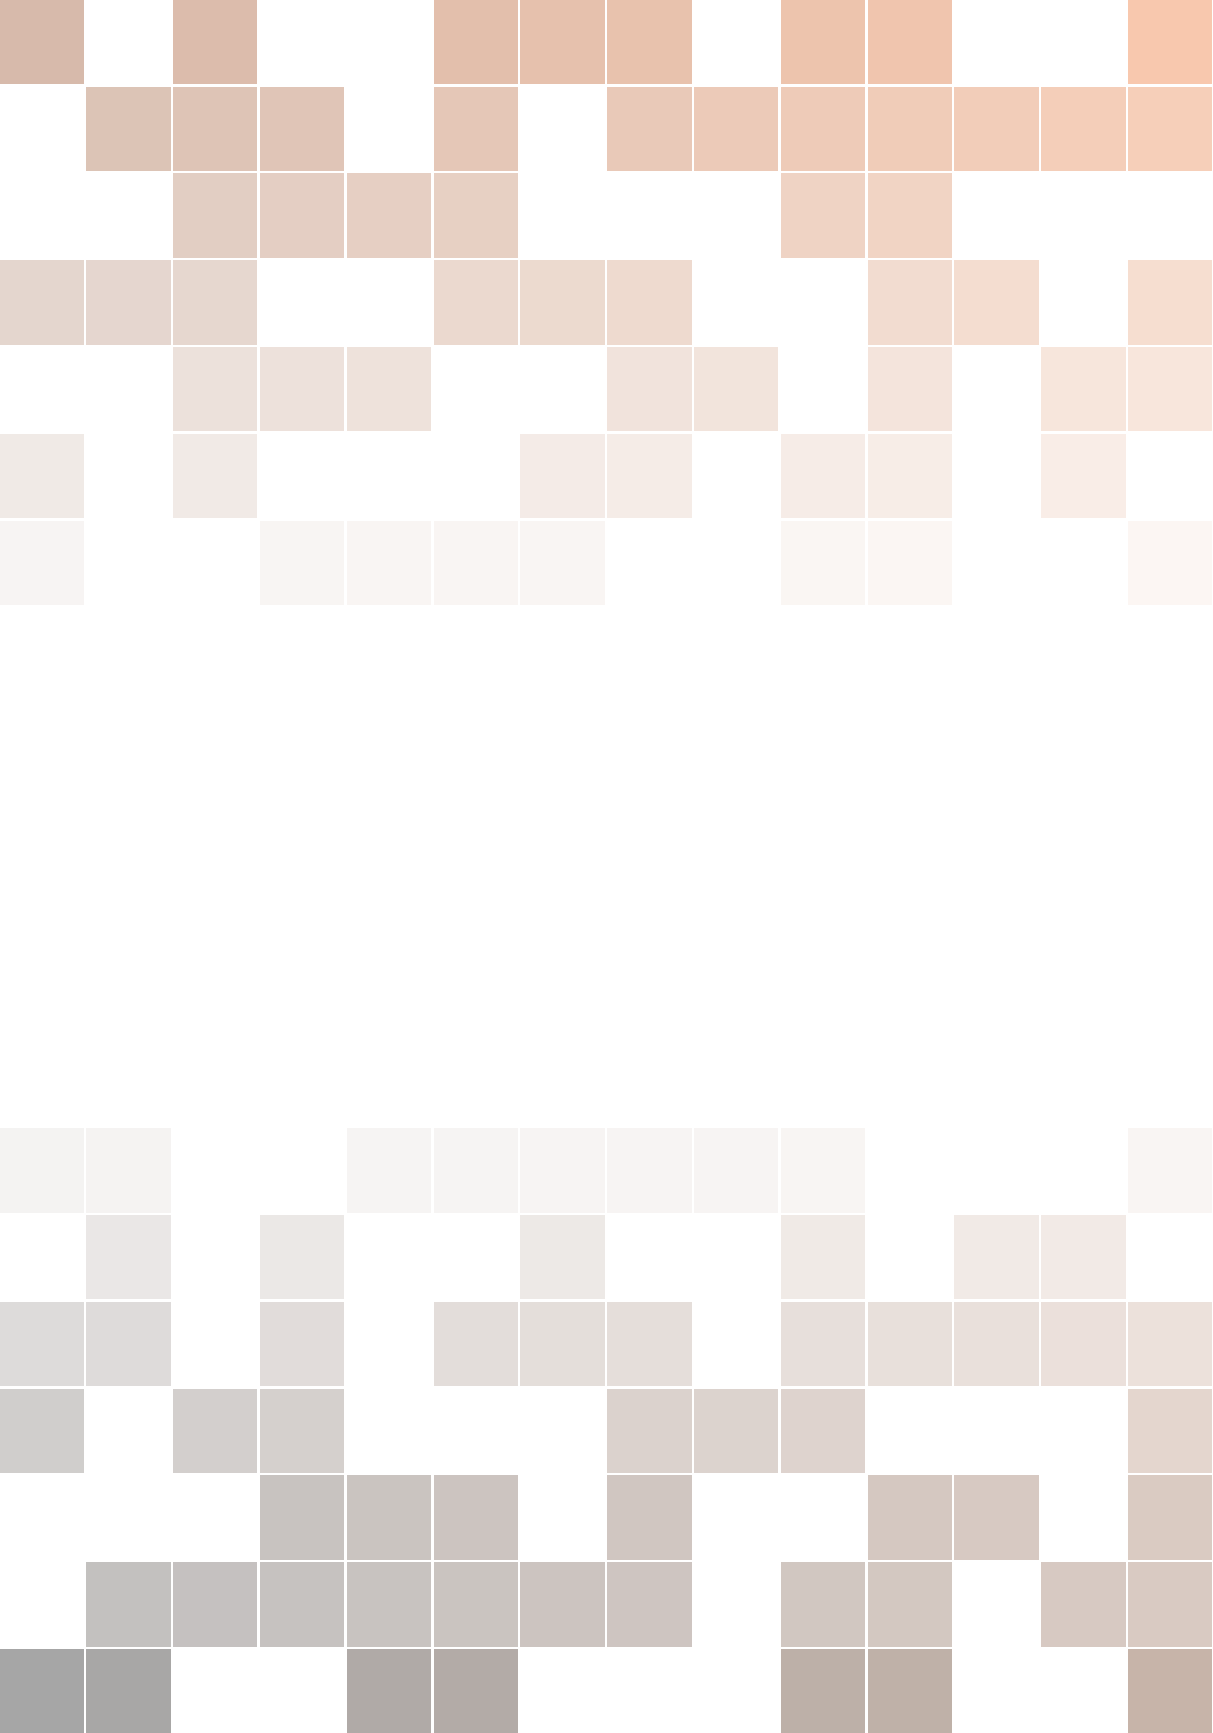
\includegraphics[width=\paperwidth]{background}}; % Background image
\draw[anchor=north] (midpoint) node [fill=ocre!30!white,fill opacity=0.6,text opacity=1,inner sep=1cm]{\Huge\centering\bfseries\sffamily\parbox[c][][t]{\paperwidth}{\centering ROAD TO DATA SCIENCE\\[15pt] % Book title
{\Large -Early Version-}\\[20pt] % Subtitle
{\huge FROM HCMUS with LOVE}}}; % Author name
\end{tikzpicture}};
\end{tikzpicture}
\vfill
\endgroup

%----------------------------------------------------------------------------------------
%	COPYRIGHT PAGE
%----------------------------------------------------------------------------------------

\newpage
~\vfill
\thispagestyle{empty}

%\noindent Copyright \copyright\ 2013 John Smith\\ % Copyright notice

%\noindent \textsc{Published by Publisher}\\ % Publisher

%\noindent \textsc{book-website.com}\\ % URL

%\noindent Licensed under the Creative Commons Attribution-NonCommercial 3.0 Unported License (the ``License''). You may not use this file except in compliance with the License. You may obtain a copy of the License at \url{http://creativecommons.org/licenses/by-nc/3.0}. Unless required by applicable law or agreed to in writing, software distributed under the License is distributed on an \textsc{``as is'' basis, without warranties or conditions of any kind}, either express or implied. See the License for the specific language governing permissions and limitations under the License.\\ % License information

%\noindent \textit{25/9/2021} % Printing/edition date

%----------------------------------------------------------------------------------------
%	TABLE OF CONTENTS
%----------------------------------------------------------------------------------------

%\usechapterimagefalse % If you don't want to include a chapter image, use this to toggle images off - it can be enabled later with \usechapterimagetrue

\chapterimage{chapter_head_1.pdf} % Table of contents heading image

\pagestyle{empty} % No headers

\tableofcontents % Print the table of contents itself

\cleardoublepage % Forces the first chapter to start on an odd page so it's on the right

\pagestyle{fancy} % Print headers again

%----------------------------------------------------------------------------------------
%	PART
%----------------------------------------------------------------------------------------

\part{DISCRETE MATHEMATICS}
    
    \chapterimage{chapter_head_1.pdf}
    
    \chapter{Propositional Logic}
        \hrule
        \vspace*{2cm}
        \normalsize
        \chudau{L}ogic là cơ sở của tất cả các suy luận toán học, nó được ứng dụng thực tiễn trong việc thiết kế hệ thống máy tính, máy học, trí tuệ nhân tạo,
        và nhiều lĩnh vực khác của khoa học máy tính cũng nhưng nhiều lĩnh vực nghiên cứu khác. 
        \pagebreak
        
        \documentclass{standalone} % Default font size and left-justified equations
\usepackage{standalone}

%----------------------------------------------------------------------------------------

%%%%%%%%%%%%%%%%%%%%%%%%%%%%%%%%%%%%%%%%%
% The Legrand Orange Book
% Structural Definitions File
% Version 2.0 (9/2/15)
%
% Original author:
% Mathias Legrand (legrand.mathias@gmail.com) with modifications by:
% Vel (vel@latextemplates.com)
% 
% This file has been downloaded from:
% http://www.LaTeXTemplates.com
%
% License:
% CC BY-NC-SA 3.0 (http://creativecommons.org/licenses/by-nc-sa/3.0/)
%
%%%%%%%%%%%%%%%%%%%%%%%%%%%%%%%%%%%%%%%%%

%----------------------------------------------------------------------------------------
%	VARIOUS REQUIRED PACKAGES AND CONFIGURATIONS
%----------------------------------------------------------------------------------------

\usepackage[top=3cm,bottom=3cm,left=3cm,right=3cm,headsep=10pt,a4paper]{geometry} % Page margins

\usepackage{graphicx} % Required for including pictures
\graphicspath{{Pictures/}} % Specifies the directory where pictures are stored

\usepackage{lipsum} % Inserts dummy text

\usepackage{tikz} % Required for drawing custom shapes

\usepackage{makecell} % Required for makeing cell in table

\usepackage[vietnamese]{babel} % English language/hyphenation

\usepackage{enumitem} % Customize lists
\setlist{nolistsep} % Reduce spacing between bullet points and numbered lists

\usepackage{booktabs} % Required for nicer horizontal rules in tables

\usepackage{xcolor} % Required for specifying colors by name
\definecolor{ocre}{RGB}{243,102,25} % Define the orange color used for highlighting throughout the book

\definecolor{darkgreen}{RGB}{0,80,0}
\usepackage{fancyhdr}
\usepackage{lettrine}
\input Acorn.fd
\newcommand*\initfamily{\usefont{U}{Acorn}{xl}{n}}
\newcommand{\chudau}[1]{%
    \lettrine[lines=3]{\initfamily\textcolor{darkgreen}{#1}}
}


%----------------------------------------------------------------------------------------
%	FONTS
%----------------------------------------------------------------------------------------

\usepackage{avant} % Use the Avantgarde font for headings
%\usepackage{times} % Use the Times font for headings
\usepackage{mathptmx} % Use the Adobe Times Roman as the default text font together with math symbols from the Sym­bol, Chancery and Com­puter Modern fonts

\usepackage{microtype} % Slightly tweak font spacing for aesthetics
\usepackage[utf8]{inputenc} % Required for including letters with accents
\usepackage[T1]{fontenc} % Use 8-bit encoding that has 256 glyphs

%----------------------------------------------------------------------------------------
%	BIBLIOGRAPHY AND INDEX
%----------------------------------------------------------------------------------------

\usepackage{csquotes}
\usepackage[style=alphabetic,citestyle=numeric,sorting=nyt,sortcites=true,autopunct=true,autolang=hyphen,hyperref=true,abbreviate=false,backref=true,backend=biber,defernumbers=true]{biblatex}
\addbibresource{bibliography.bib} % BibTeX bibliography file
\defbibheading{bibempty}{}

\usepackage{calc} % For simpler calculation - used for spacing the index letter headings correctly
\usepackage{makeidx} % Required to make an index
\makeindex % Tells LaTeX to create the files required for indexing

%----------------------------------------------------------------------------------------
%	MAIN TABLE OF CONTENTS
%----------------------------------------------------------------------------------------

\usepackage{titletoc} % Required for manipulating the table of contents

\contentsmargin{0cm} % Removes the default margin

% Part text styling
\titlecontents{part}[0cm]
{\addvspace{20pt}\centering\large\bfseries}
{}
{}
{}

% Chapter text styling
\titlecontents{chapter}[1.25cm] % Indentation
{\addvspace{12pt}\large\sffamily\bfseries} % Spacing and font options for chapters
{\color{ocre!60}\contentslabel[\Large\thecontentslabel]{1.25cm}\color{ocre}} % Chapter number
{\color{ocre}}  
{\color{ocre!60}\normalsize\;\titlerule*[.5pc]{.}\;\thecontentspage} % Page number

% Section text styling
\titlecontents{section}[1.25cm] % Indentation
{\addvspace{3pt}\sffamily\bfseries} % Spacing and font options for sections
{\contentslabel[\thecontentslabel]{1.25cm}} % Section number
{}
{\hfill\color{black}\thecontentspage} % Page number
[]

% Subsection text styling
\titlecontents{subsection}[1.25cm] % Indentation
{\addvspace{1pt}\sffamily\small} % Spacing and font options for subsections
{\contentslabel[\thecontentslabel]{1.25cm}} % Subsection number
{}
{\ \titlerule*[.5pc]{.}\;\thecontentspage} % Page number
[]

% List of figures
\titlecontents{figure}[0em]
{\addvspace{-5pt}\sffamily}
{\thecontentslabel\hspace*{1em}}
{}
{\ \titlerule*[.5pc]{.}\;\thecontentspage}
[]

% List of tables
\titlecontents{table}[0em]
{\addvspace{-5pt}\sffamily}
{\thecontentslabel\hspace*{1em}}
{}
{\ \titlerule*[.5pc]{.}\;\thecontentspage}
[]

%----------------------------------------------------------------------------------------
%	MINI TABLE OF CONTENTS IN PART HEADS
%----------------------------------------------------------------------------------------

% Chapter text styling
\titlecontents{lchapter}[0em] % Indenting
{\addvspace{15pt}\large\sffamily\bfseries} % Spacing and font options for chapters
{\color{ocre}\contentslabel[\Large\thecontentslabel]{1.25cm}\color{ocre}} % Chapter number
{}  
{\color{ocre}\normalsize\sffamily\bfseries\;\titlerule*[.5pc]{.}\;\thecontentspage} % Page number

% Section text styling
\titlecontents{lsection}[0em] % Indenting
{\sffamily\small} % Spacing and font options for sections
{\contentslabel[\thecontentslabel]{1.25cm}} % Section number
{}
{}

% Subsection text styling
\titlecontents{lsubsection}[.5em] % Indentation
{\normalfont\footnotesize\sffamily} % Font settings
{}
{}
{}

%----------------------------------------------------------------------------------------
%	PAGE HEADERS
%----------------------------------------------------------------------------------------

%\usepackage{fancyhdr} % Required for header and footer configuration

\pagestyle{fancy}
\renewcommand{\chaptermark}[1]{\markboth{\sffamily\normalsize\bfseries\chaptername\ \thechapter.\ #1}{}} % Chapter text font settings
\renewcommand{\sectionmark}[1]{\markright{\sffamily\normalsize\thesection\hspace{5pt}#1}{}} % Section text font settings
\fancyhf{} \fancyhead[LE,RO]{\sffamily\normalsize\thepage} % Font setting for the page number in the header
\fancyhead[LO]{\rightmark} % Print the nearest section name on the left side of odd pages
\fancyhead[RE]{\leftmark} % Print the current chapter name on the right side of even pages
\renewcommand{\headrulewidth}{0.5pt} % Width of the rule under the header
\addtolength{\headheight}{2.5pt} % Increase the spacing around the header slightly
\renewcommand{\footrulewidth}{0pt} % Removes the rule in the footer
\fancypagestyle{plain}{\fancyhead{}\renewcommand{\headrulewidth}{0pt}} % Style for when a plain pagestyle is specified

% Removes the header from odd empty pages at the end of chapters
\makeatletter
\renewcommand{\cleardoublepage}{
\clearpage\ifodd\c@page\else
\hbox{}
\vspace*{\fill}
\thispagestyle{empty}
\newpage
\fi}

%----------------------------------------------------------------------------------------
%	THEOREM STYLES
%----------------------------------------------------------------------------------------

\usepackage{amsmath,amsfonts,amssymb,amsthm} % For math equations, theorems, symbols, etc

\newcommand{\intoo}[2]{\mathopen{]}#1\,;#2\mathclose{[}}
\newcommand{\ud}{\mathop{\mathrm{{}d}}\mathopen{}}
\newcommand{\intff}[2]{\mathopen{[}#1\,;#2\mathclose{]}}
\newtheorem{notation}{Notation}[chapter]

% Boxed/framed environments
\newtheoremstyle{ocrenumbox}% % Theorem style name
{0pt}% Space above
{0pt}% Space below
{\normalfont}% % Body font
{}% Indent amount
{\small\bf\sffamily\color{ocre}}% % Theorem head font
{\;}% Punctuation after theorem head
{0.25em}% Space after theorem head
{\small\sffamily\color{ocre}\thmname{#1}\nobreakspace\thmnumber{\@ifnotempty{#1}{}\@upn{#2}}% Theorem text (e.g. Theorem 2.1)
\thmnote{\nobreakspace\the\thm@notefont\sffamily\bfseries\color{black}---\nobreakspace#3.}} % Optional theorem note
\renewcommand{\qedsymbol}{$\blacksquare$}% Optional qed square

\newtheoremstyle{blacknumex}% Theorem style name
{5pt}% Space above
{5pt}% Space below
{\normalfont}% Body font
{} % Indent amount
{\small\bf\sffamily}% Theorem head font
{\;}% Punctuation after theorem head
{0.25em}% Space after theorem head
{\small\sffamily{\tiny\ensuremath{\blacksquare}}\nobreakspace\thmname{#1}\nobreakspace\thmnumber{\@ifnotempty{#1}{}\@upn{#2}}% Theorem text (e.g. Theorem 2.1)
\thmnote{\nobreakspace\the\thm@notefont\sffamily\bfseries---\nobreakspace#3.}}% Optional theorem note

\newtheoremstyle{blacknumbox} % Theorem style name
{0pt}% Space above
{0pt}% Space below
{\normalfont}% Body font
{}% Indent amount
{\small\bf\sffamily}% Theorem head font
{\;}% Punctuation after theorem head
{0.25em}% Space after theorem head
{\small\sffamily\thmname{#1}\nobreakspace\thmnumber{\@ifnotempty{#1}{}\@upn{#2}}% Theorem text (e.g. Theorem 2.1)
\thmnote{\nobreakspace\the\thm@notefont\sffamily\bfseries---\nobreakspace#3.}}% Optional theorem note

% Non-boxed/non-framed environments
\newtheoremstyle{ocrenum}% % Theorem style name
{5pt}% Space above
{5pt}% Space below
{\normalfont}% % Body font
{}% Indent amount
{\small\bf\sffamily\color{ocre}}% % Theorem head font
{\;}% Punctuation after theorem head
{0.25em}% Space after theorem head
{\small\sffamily\color{ocre}\thmname{#1}\nobreakspace\thmnumber{\@ifnotempty{#1}{}\@upn{#2}}% Theorem text (e.g. Theorem 2.1)
\thmnote{\nobreakspace\the\thm@notefont\sffamily\bfseries\color{black}---\nobreakspace#3.}} % Optional theorem note
\renewcommand{\qedsymbol}{$\blacksquare$}% Optional qed square
\makeatother

% Defines the theorem text style for each type of theorem to one of the three styles above
\newcounter{dummy} 
\numberwithin{dummy}{section}
\theoremstyle{ocrenumbox}
\newtheorem{theoremeT-nono}[dummy]{}
\newtheorem{problem}{Problem}[chapter]
\newtheorem{exerciseT}{Bài tập}[chapter]
\theoremstyle{blacknumex}
\newtheorem{exampleT}{Ví dụ}[chapter]
\theoremstyle{blacknumbox}
\newtheorem{vocabulary}{Vocabulary}[chapter]
\newtheorem{definitionT}{Định nghĩa}[section]
\newtheorem{corollaryT}[dummy]{Hệ quả}
\theoremstyle{ocrenum}
\newtheorem{proposition}[dummy]{Chứng minh}

%----------------------------------------------------------------------------------------
%	DEFINITION OF COLORED BOXES
%----------------------------------------------------------------------------------------

\RequirePackage[framemethod=default]{mdframed} % Required for creating the theorem, definition, exercise and corollary boxes

% Theorem box
\newmdenv[skipabove=7pt,
skipbelow=7pt,
backgroundcolor=black!5,
linecolor=ocre,
innerleftmargin=5pt,
innerrightmargin=5pt,
innertopmargin=5pt,
leftmargin=0cm,
rightmargin=0cm,
innerbottommargin=5pt]{tBox}

% Exercise box	  
\newmdenv[skipabove=7pt,
skipbelow=7pt,
rightline=false,
leftline=true,
topline=false,
bottomline=false,
backgroundcolor=ocre!10,
linecolor=ocre,
innerleftmargin=5pt,
innerrightmargin=5pt,
innertopmargin=5pt,
innerbottommargin=5pt,
leftmargin=0cm,
rightmargin=0cm,
linewidth=4pt]{eBox}	

% Definition box
\newmdenv[skipabove=7pt,
skipbelow=7pt,
rightline=false,
leftline=true,
topline=false,
bottomline=false,
linecolor=ocre,
innerleftmargin=5pt,
innerrightmargin=5pt,
innertopmargin=0pt,
leftmargin=0cm,
rightmargin=0cm,
linewidth=4pt,
innerbottommargin=0pt]{dBox}	

%my definition box
\newmdenv[skipabove=7pt,
skipbelow=7pt,
backgroundcolor=blue!2,
linecolor=ocre,
innerleftmargin=5pt,
innerrightmargin=5pt,
innertopmargin=5pt,
leftmargin=0cm,
rightmargin=0cm,
innerbottommargin=5pt]{ttBox}

% Corollary box
\newmdenv[skipabove=7pt,
skipbelow=7pt,
rightline=false,
leftline=true,
topline=false,
bottomline=false,
linecolor=gray,
backgroundcolor=black!5,
innerleftmargin=5pt,
innerrightmargin=5pt,
innertopmargin=5pt,
leftmargin=0cm,
rightmargin=0cm,
linewidth=4pt,
innerbottommargin=5pt]{cBox}

% Creates an environment for each type of theorem and assigns it a theorem text style from the "Theorem Styles" section above and a colored box from above
\newenvironment{theorem}{\begin{tBox}\begin{theoremeT}}{\end{theoremeT}\end{tBox}}
\newenvironment{exercise}{\begin{eBox}\begin{exerciseT}}{\hfill{\color{ocre}\tiny\ensuremath{\blacksquare}}\end{exerciseT}\end{eBox}}				  
\newenvironment{definition}{\begin{ttBox}\begin{definitionT}}{\end{definitionT}\end{ttBox}}	
\newenvironment{example}{\begin{exampleT}}{\hfill{\tiny\ensuremath{\blacksquare}}\end{exampleT}}		
\newenvironment{corollary}{\begin{cBox}\begin{corollaryT}}{\end{corollaryT}\end{cBox}}	

%----------------------------------------------------------------------------------------
%	REMARK ENVIRONMENT
%----------------------------------------------------------------------------------------

\newenvironment{remark}{\par\vspace{10pt}\small % Vertical white space above the remark and smaller font size
\begin{list}{}{
\leftmargin=35pt % Indentation on the left
\rightmargin=25pt}\item\ignorespaces % Indentation on the right
\makebox[-2.5pt]{\begin{tikzpicture}[overlay]
\node[draw=ocre!60,line width=1pt,circle,fill=ocre!25,font=\sffamily\bfseries,inner sep=2pt,outer sep=0pt] at (-15pt,0pt){\textcolor{ocre}{R}};\end{tikzpicture}} % Orange R in a circle
\advance\baselineskip -1pt}{\end{list}\vskip5pt} % Tighter line spacing and white space after remark

%----------------------------------------------------------------------------------------
%	SECTION NUMBERING IN THE MARGIN
%----------------------------------------------------------------------------------------

\makeatletter
\renewcommand{\@seccntformat}[1]{\llap{\textcolor{ocre}{\csname the#1\endcsname}\hspace{1em}}}                    
\renewcommand{\section}{\@startsection{section}{1}{\z@}
{-4ex \@plus -1ex \@minus -.4ex}
{1ex \@plus.2ex }
{\normalfont\large\sffamily\bfseries}}
\renewcommand{\subsection}{\@startsection {subsection}{2}{\z@}
{-3ex \@plus -0.1ex \@minus -.4ex}
{0.5ex \@plus.2ex }
{\normalfont\sffamily\bfseries}}
\renewcommand{\subsubsection}{\@startsection {subsubsection}{3}{\z@}
{-2ex \@plus -0.1ex \@minus -.2ex}
{.2ex \@plus.2ex }
{\normalfont\small\sffamily\bfseries}}                        
\renewcommand\paragraph{\@startsection{paragraph}{4}{\z@}
{-2ex \@plus-.2ex \@minus .2ex}
{.1ex}
{\normalfont\small\sffamily\bfseries}}

%----------------------------------------------------------------------------------------
%	PART HEADINGS
%----------------------------------------------------------------------------------------

% numbered part in the table of contents
\newcommand{\@mypartnumtocformat}[2]{%
\setlength\fboxsep{0pt}%
\noindent\colorbox{ocre!20}{\strut\parbox[c][.7cm]{\ecart}{\color{ocre!70}\Large\sffamily\bfseries\centering#1}}\hskip\esp\colorbox{ocre!40}{\strut\parbox[c][.7cm]{\linewidth-\ecart-\esp}{\Large\sffamily\centering#2}}}%
%%%%%%%%%%%%%%%%%%%%%%%%%%%%%%%%%%
% unnumbered part in the table of contents
\newcommand{\@myparttocformat}[1]{%
\setlength\fboxsep{0pt}%
\noindent\colorbox{ocre!40}{\strut\parbox[c][.7cm]{\linewidth}{\Large\sffamily\centering#1}}}%
%%%%%%%%%%%%%%%%%%%%%%%%%%%%%%%%%%
\newlength\esp
\setlength\esp{4pt}
\newlength\ecart
\setlength\ecart{1.2cm-\esp}
\newcommand{\thepartimage}{}%
\newcommand{\partimage}[1]{\renewcommand{\thepartimage}{#1}}%
\def\@part[#1]#2{%
\ifnum \c@secnumdepth >-2\relax%
\refstepcounter{part}%
\addcontentsline{toc}{part}{\texorpdfstring{\protect\@mypartnumtocformat{\thepart}{#1}}{\partname~\thepart\ ---\ #1}}
\else%
\addcontentsline{toc}{part}{\texorpdfstring{\protect\@myparttocformat{#1}}{#1}}%
\fi%
\startcontents%
\markboth{}{}%
{\thispagestyle{empty}%
\begin{tikzpicture}[remember picture,overlay]%
\node at (current page.north west){\begin{tikzpicture}[remember picture,overlay]%	
\fill[ocre!20](0cm,0cm) rectangle (\paperwidth,-\paperheight);
\node[anchor=north] at (4cm,-3.25cm){\color{ocre!40}\fontsize{220}{100}\sffamily\bfseries\@Roman\c@part}; 
\node[anchor=south east] at (\paperwidth-1cm,-\paperheight+1cm){\parbox[t][][t]{8.5cm}{
\printcontents{l}{0}{\setcounter{tocdepth}{1}}%
}};
\node[anchor=north east] at (\paperwidth-1.5cm,-3.25cm){\parbox[t][][t]{15cm}{\strut\raggedleft\color{white}\fontsize{30}{30}\sffamily\bfseries#2}};
\end{tikzpicture}};
\end{tikzpicture}}%
\@endpart}
\def\@spart#1{%
\startcontents%
\phantomsection
{\thispagestyle{empty}%
\begin{tikzpicture}[remember picture,overlay]%
\node at (current page.north west){\begin{tikzpicture}[remember picture,overlay]%	
\fill[ocre!20](0cm,0cm) rectangle (\paperwidth,-\paperheight);
\node[anchor=north east] at (\paperwidth-1.5cm,-3.25cm){\parbox[t][][t]{15cm}{\strut\raggedleft\color{white}\fontsize{30}{30}\sffamily\bfseries#1}};
\end{tikzpicture}};
\end{tikzpicture}}
\addcontentsline{toc}{part}{\texorpdfstring{%
\setlength\fboxsep{0pt}%
\noindent\protect\colorbox{ocre!40}{\strut\protect\parbox[c][.7cm]{\linewidth}{\Large\sffamily\protect\centering #1\quad\mbox{}}}}{#1}}%
\@endpart}
\def\@endpart{\vfil\newpage
\if@twoside
\if@openright
\null
\thispagestyle{empty}%
\newpage
\fi
\fi
\if@tempswa
\twocolumn
\fi}

%----------------------------------------------------------------------------------------
%	CHAPTER HEADINGS
%----------------------------------------------------------------------------------------

% A switch to conditionally include a picture, implemented by  Christian Hupfer
\newif\ifusechapterimage
\usechapterimagetrue
\newcommand{\thechapterimage}{}%
\newcommand{\chapterimage}[1]{\ifusechapterimage\renewcommand{\thechapterimage}{#1}\fi}%
\def\@makechapterhead#1{%
{\parindent \z@ \raggedright \normalfont
\ifnum \c@secnumdepth >\m@ne
\if@mainmatter
\begin{tikzpicture}[remember picture,overlay]
\node at (current page.north west)
{\begin{tikzpicture}[remember picture,overlay]
\node[anchor=north west,inner sep=0pt] at (0,0) {\ifusechapterimage\includegraphics[width=\paperwidth]{\thechapterimage}\fi};
\draw[anchor=west] (\Gm@lmargin,-9cm) node [line width=2pt,rounded corners=15pt,draw=ocre,fill=white,fill opacity=0.5,inner sep=15pt]{\strut\makebox[22cm]{}};
\draw[anchor=west] (\Gm@lmargin+.3cm,-9cm) node {\huge\sffamily\bfseries\color{black}\thechapter. #1\strut};
\end{tikzpicture}};
\end{tikzpicture}
\else
\begin{tikzpicture}[remember picture,overlay]
\node at (current page.north west)
{\begin{tikzpicture}[remember picture,overlay]
\node[anchor=north west,inner sep=0pt] at (0,0) {\ifusechapterimage\includegraphics[width=\paperwidth]{\thechapterimage}\fi};
\draw[anchor=west] (\Gm@lmargin,-9cm) node [line width=2pt,rounded corners=15pt,draw=ocre,fill=white,fill opacity=0.5,inner sep=15pt]{\strut\makebox[22cm]{}};
\draw[anchor=west] (\Gm@lmargin+.3cm,-9cm) node {\huge\sffamily\bfseries\color{black}#1\strut};
\end{tikzpicture}};
\end{tikzpicture}
\fi\fi\par\vspace*{270\p@}}}

%-------------------------------------------

\def\@makeschapterhead#1{%
\begin{tikzpicture}[remember picture,overlay]
\node at (current page.north west)
{\begin{tikzpicture}[remember picture,overlay]
\node[anchor=north west,inner sep=0pt] at (0,0) {\ifusechapterimage\includegraphics[width=\paperwidth]{\thechapterimage}\fi};
\draw[anchor=west] (\Gm@lmargin,-9cm) node [line width=2pt,rounded corners=15pt,draw=ocre,fill=white,fill opacity=0.5,inner sep=15pt]{\strut\makebox[22cm]{}};
\draw[anchor=west] (\Gm@lmargin+.3cm,-9cm) node {\huge\sffamily\bfseries\color{black}#1\strut};
\end{tikzpicture}};
\end{tikzpicture}
\par\vspace*{270\p@}}
\makeatother

%----------------------------------------------------------------------------------------
%	HYPERLINKS IN THE DOCUMENTS
%----------------------------------------------------------------------------------------

\usepackage{hyperref}
\hypersetup{hidelinks,colorlinks=false,breaklinks=true,urlcolor= ocre,bookmarksopen=false,pdftitle={Title},pdfauthor={Author}}
\usepackage{bookmark}
\bookmarksetup{
open,
numbered,
addtohook={%
\ifnum\bookmarkget{level}=0 % chapter
\bookmarksetup{bold}%
\fi
\ifnum\bookmarkget{level}=-1 % part
\bookmarksetup{color=ocre,bold}%
\fi
}
}

 % Insert the commands.tex file which contains the majority of the structure behind the template

\begin{document}

    \section{Mệnh đề - các phép toán với mệnh đề}
    \subsection{Mệnh đề}
    \begin{theorem} \index{Mệnh đề}
        \emph{Mệnh đề} là một khẳng định có chân trị xác định, có thể đúng hoặc sai nhưng không thể vừa đúng vừa sai.
    \end{theorem}
        \begin{example}
            Những ví dụ sau đều là mệnh đề.
            \begin{enumerate}
                \item Hà Nội là thủ đô của Việt Nam.
                \item Thành phố Hồ Chí Minh là vùng trồng lúc lớn nhất Đông Nam Á.
                \item $1 + 1 = 2$.
                \item $5 - 5 = 10$.
            \end{enumerate}
        \end{example}
        Trong đó mệnh đề 1 và 3 là mệnh đề đúng, mệnh đề 2 và 4 là mệnh đề sai.\\
        \begin{example}
            Xét những ví dụ sau.
            \begin{enumerate}
                \item Hôm nay là thứ mấy?
                \item Hãy chăm chỉ học hành.
                \item $x + 1 = 2$.
                \item $x + y = z$.
            \end{enumerate}
        \end{example}

        Hai ví dụ đầu tiên không phải là mệnh đề vì không phải là câu khẳng định. Hai ví dụ 3 và 4 không phải là một mệnh đề vì không có chân trị xác
        định, có thể đúng hoặc sai. Lưu ý rằng ví dụ 3 và 4 có thể trở thành một mệnh đề khi ta xác định giá của của các biến thành phần.

        Chúng ta sử dụng các chữ cái để biểu thị các \emph{biến mệnh đề}, nghĩa là biến đại diện cho các mệnh đề, cũng giống như các chữ cái được dùng
        để đại diện cho các biến số. Các chữ cái thường được dùng để quy ước cho các biến mệnh đề là $p, q, r, s, ...$. Chân trị của một mệnh đề đúng, được kí hiệu là
        $T$, nếu đó là một mệnh đề đúng và chân trị của một mệnh đề sai, được kí hiệu là $F$, nếu đó là một mệnh đề sai.

        \begin{theorem}\index{Các loại mệnh đề}
            Có hai loại mệnh đề:
            \begin{itemize}
                \item \emph{Mệnh đề phức hợp} là những mệnh đề được xây dựng bằng cách kết hợp một hoặc nhiều mệnh đề với các toán tử logic, hay nói cách khác
                là liên kết bằng các liên từ: \textit{và, hay, nếu, thì ...} hoặc trạng từ \textit{không}.
                \item \emph{Mệnh đề nguyên thủy (sơ cấp)} là mệnh đề không thể xây dựng bằng cách kết hợp một hoặc nhiều mệnh đề với các toán tử logic.
            \end{itemize}
        \end{theorem}
        \begin{example} Xét những ví dụ sau.
            \begin{enumerate}
                \item 2 là số nguyên tố. \textit{(mệnh đề nguyên thủy)}
                \item Việt Nam có lãnh thổ hình chữ S. \textit{(mệnh đề nguyên thủy)}
                \item Nếu $1 + 1 = 2$ thì $1$ là số nguyên tố. \textit{(mệnh đề phức hợp)}
            \end{enumerate}
        \end{example}
    \subsection{Phép phủ định} \index{Phép phủ định}
        \begin{definition}
            Cho mệnh đề $p$, mệnh đề phủ định của $p$ được ký hiệu là $\neg p$ (hoặc cũng có thể ký hiệu là $\overline{p}$) được đọc là "không $p$" hay "phủ định của $p$".
            Chân trị của $\neg p$ có giá trị ngược lại so với chân trị của $p$.
        \end{definition}
        \begin{table}[ht]
            \centering
            \setlength{\tabcolsep}{18pt}
            \begin{tabular}{c c}
                $p$  & $\neg p$\\
                \hline
                1 & 0\\
                0 & 1
            \end{tabular}
            \caption{Bảng chân trị $\neg p$}
        \end{table}
        \begin{example}\ \\
            $\begin{array}{l l}
                p &=  \text{"PC của Hào chạy hệ điều hành Linux".}\\
                \neg p &=  \text{"PC của Hào không chạy hệ điều hành Linux".}
            \end{array}$
        \end{example}
    \subsection{Phép nối liền} \index{Phép nối liền}
        \begin{definition}
            Cho hai mệnh đề $p$ và $q$. Phép nối liền $p$ và $q$ được ký hiệu là $p\land q$ được đọc là" $p$ và $q$" (hoặc "$p$ hội $q$"). $p \land q$ có chân trị đúng khi cả $p$ và $q$ đều đúng.
        \end{definition}
        \begin{table}[h!]
            \centering
            \setlength{\tabcolsep}{18pt}
            \begin{tabular}{c c c}
                $p$ & $q$ & $p \land q$\\ \hline
                0 & 0 & 0\\ 
                0 & 1 & 0\\
                1 & 0 & 0\\
                1 & 1 & 1
            \end{tabular}
            \caption{Bảng chân trị $p \land q$}
        \end{table}
        
        Lưu ý rằng trong toán logic, đôi khi từ "nhưng" được sử dụng thay thế cho từ "và". Ví dụ như câu nói "Mặt trời đang sáng, nhưng trời đang mưa" là một cách nói khác của câu "Mặt trời đang sáng và trời đang mưa". Trong ngôn ngữ tự nhiên "và" và "nhưng" có thể mang ý nghĩa khác nhau nhưng chúng ta sẽ không quan tâm đến vấn đề đó ở đây.
        
        \begin{example}\ \\
            $\begin{array}{l l}
                p &= \text{"Toán rời rạc là một môn không khó".}\\
                q &= \text{"Giáo viên dạy môn toán rời rạc rất dễ thương:3".}\\
                p \land q &= \text{"Toán rời rạc mà một môn không khó và giáo viên dạy rất dễ thương:3".}
            \end{array}$
        \end{example}
        
        \begin{example}  Xét những ví dụ sau.
            \begin{enumerate}
                \item 2 là số chẵn và 2 là số nguyên tố.(mệnh đề đúng)
                \item 1 + 1 = 3 nhưng 2 + 2 = 4.(mệnh đề sai) \footnote{
                    1 + 1 = 3 là một mệnh đề sai còn 2 + 2 = 4 là một mệnh đề đúng, do đó đây là một mệnh đề sai.
                }
            \end{enumerate}
        \end{example}
    \subsection{Phép nối rời} \index{phép nối rời}
        \begin{definition}
            Cho hai mệnh đề $p$ và $q$. Phép nối rời $p$ và $q$ được ký hiệu là $p \lor q$ được đọc là "$p$ hay $q$" (hoặc "$p$ tuyển $q$"). $p \lor q$ có chân trị đúng khi một trong hai hoặc cả hai đều có chân trị đúng.
        \end{definition}
        \begin{table}[h!]
            \centering
            \setlength{\tabcolsep}{18pt}
            \begin{tabular}{c c c}
                $p$ & $q$ & $p \lor q$ \\ \hline
                0 & 0 & 0\\ 
                0 & 1 & 1\\
                1 & 0 & 1\\
                1 & 1 & 1
            \end{tabular}
            \caption{Bảng chân trị $p \lor q$}
        \end{table}
        
        \begin{example} Nhân dịp 20/10\\
            $\begin{array}{l l}
                p &= \text{"Bạn sẽ mua quà cho Linh".}\\
                q &= \text{"Bạn sẽ mua quà cho Lan".}\\
                p \lor q &= \text{"Bạn sẽ mua quà cho Linh hay Lan (hoặc cả hai)".}
            \end{array}$
        \end{example}
        
        Đưa ví dụ trên vào ngữ cảnh thực tế, bạn có thể lựa chọn mua quà cho Linh hay cho Lan hay sẽ mua cho cả hai. Trong trường hợp này sử dụng từ "hay" sẽ hợp lý hơn "hoặc", "hay" mang ý nghĩa một trong hai hay cả hai trong khi từ "hoặc" sẽ mang thiên hướng một trong hai nhưng không phải cả hai\footnote{
            Trong tiếng anh có hai cách từ "or" được sử dụng: \textbf{inclusive or} nghĩa là một trong hai hay cả hai và \textbf{exclusive or} nghĩa là chỉ một trong hai.
        }.
        
        \begin{definition} \index{Phép tuyển loại}
            Cho hai mệnh đề $p$ và $q$. Phép tuyển loại $p$ hoặc $q$ được ký hiệu là $p \oplus q$ được đọc là "$p$ hoặc $q$". $p \oplus q$ có chân trị đúng khi chỉ có chính xác một trong $p$ hoặc $q$ có chân trị đúng.
        \end{definition}
        \begin{table}[h!]
            \centering
            \setlength{\tabcolsep}{18pt}
            \begin{tabular}{c c c}
                $p$ & $q$ & $p \oplus q$ \\ \hline
                0 & 0 & 0\\
                0 & 1 & 1\\
                1 & 0 & 1\\ 
                1 & 1 & 0
            \end{tabular}
            \caption{Bảng chân trị $p \oplus q$}
        \end{table}
        
        \begin{example}\ \\
            $\begin{array}{l l}
                p &= \text{"Bạn sẽ thi tổ hợp KHTN".}\\
                q &= \text{"Bạn sẽ thi tổ hợp KHXH".}\\
                p \lor q &= \text{"Bạn sẽ thi tổ hợp KHTN hoặc KHXH".}
            \end{array}$
        \end{example}
        
        Ví dụ trên dựa trên kỳ thi TPHTQG năm 2021, do cả hai bài thi tổ hợp đều thi trong cùng một buối nên thí sinh chỉ có thể chọn một trong hai chứ không thể chọn cả hai được. Tương tự với câu "Miễn phí cơm thêm hoặc dưa chua", bạn sẽ chỉ có thể lựa chọn cơm thêm hoặc dưa chua kèm với món ăn chính hoặc phải trả thêm tiền để có thể mua cả hai.
    \subsection{Phép kéo theo} \index{Phép kéo theo}
        \begin{definition}
            Cho hai mệnh đề $p$ và $q$. Phép kéo theo $p \to q$ là mệnh đề "nếu $p$ thì $q$". $p \to q$ có chân trị sai khi $q$ đúng và $q$ sai. $p$ được gọi là điều kiện đủ của $q$ còn $q$ được gọi là điều kiện cần của $p$.
        \end{definition}
        \begin{table}[h!]
            \centering
            \setlength{\tabcolsep}{18pt}
            \begin{tabular}{c c c}
                $p$ & $q$ & $p \to q$ \\ \hline
                0 & 0 & 1\\
                0 & 1 & 1\\ 
                1 & 0 & 0\\
                1 & 1 & 1
            \end{tabular}
            \caption{Bảng chân trị $p \to q$}
        \end{table}
        
        \begin{table}[h!]
            \centering
            \setlength{\tabcolsep}{20pt}
            \caption{Một số cách diễn đạt khác nhau của $p \to q$}
            \begin{tabular}{c|c}
                \hline
                Nếu $p$, thì $q$ & $p$ suy ra $q$\\
                Nếu $p$,$q$ & $p$ chỉ khi $q$ \\
                $p$ là điều kiện đủ của $q$ & Điều kiện đủ cho $q$ là $p$\\
                $q$ nếu $p$ & $q$ bất cứ khi nào $p$\\
                $q$ khi $p$ & $q$ là điều kiện cần của $p$\\
                Điều kiện cần của $p$ là $q$ & $q$ theo sau $p$\\
                $q$ trừ khi $\neg p$ &
            \end{tabular}
        \end{table}
        
        Một cách hữu ích để hiểu chân trị của mệnh đề trên là nghĩ về một hợp đồng hoặc cam kết. Ví dụ khi một chính trị gia ra tranh cử, ông cam kết rằng:
        \begin{center}
            "Nếu tôi được bầu, tôi sẽ giảm thuế."\\
        \end{center}
        Nếu chính trị gia trên đắc cử, cử tri sẽ mong đợi được giảm thuế. Tuy nhiên nếu chính trị gia trên thất cử, cử tri sẽ không thể kỳ vọng được giảm thuế dù có thể với tầm ảnh hưởng của chính trị gia đó và sự ủng hộ người dân có thể yêu cầu chính quyền đương nhiệm giảm thuế. Chỉ khi chính trị gia đó đắc cử nhưng không giảm thuế thì cử tri mới có thể nói rằng vị chính trị gia đó đã phá vỡ cam kết khi tranh cử. Kịch bản cuối cùng này tương ứng với trường hợp $q$ đúng nhưng $p$ sai trong mệnh đề $p \to q$.
        
        Tương tự hãy xen xét một lời hứa của một giáo sư:
        \begin{center}
            "Nếu em làm hết bài tập, thầy sẽ cho em 10 điểm".
        \end{center}
        
        Nếu bạn làm được hết bài tập, bạn sẽ được 10 điểm. Nếu không thể hoàn thành tất cả bài tập nhưng dựa trên sự chăm chỉ và năng nổ phát biểu xây dựng bài, vị giáo sư đó có thể vẫn sẽ chon bạn 10 điểm. Tuy nhiên nếu bạn làm được hết bài tập mà bạn vẫn không được 10 điểm, bạn sẽ cảm thấy bị lừa và vị giáo sư kia đã thất hứa.
        
        Trong số các cách khác nhau để diễn đạt $p \to q$, hai cách dễ bị nhầm lẫn nhất là" $p$ chỉ khi $q$" và "$q$ trừ khi $\neg p$".
        
        Để nhớ rằng "$p$ chỉ khi $q$" diễn đạt ý nghĩa tương tự với "Nếu $q$ thì $p$", cần nhớ rằng "$p$ chỉ khi $q$" nói rằng $p$ không thể đúng khi $q$ không đúng. Tức là mệnh đề $p \to q$ không thể đúng nếu $p$ đúng nhưng $q$ lại sai. Khi $p$ sai, $p$ có thể đúng hoặc sai do mệnh đề trên không nói lên điều gì về giá trị chân lý của $q$. Chúng ta không sử dụng "$q$ khi chỉ $p$" để diễn đạt $p \to q$ vì điều này không đúng. Để thấy được điều này, để ý rằng chân trị của "$p$ chỉ khi $p$" và $p \to q$ khác nhau khi $p$ và $q$ có chân trị khác nhau.
        
        Để nhớ rằng "$q$ trừ khi $\neg p$" diễn đạt ý nghĩa tương tự "Nếu $p$, thì $q$", cần nhớ rằng "$q$ trừ khi $\neg p$" có nghĩa là nếu $\neg p$ sai thì $q$ phải đúng. Đó là mệnh đề "$q$ trừ khi $\neg p$" sai khi $p$ đúng nhưng $q$ sai, nhưng ngược lại thì đúng. Hệ quả là "$q$ trừ khi $p$" và $p \to q$ luôn có cùng chân trị.
        
        \begin{example}\ \\
            $\begin{array}{l l}
                p &= \text{"Sơn đẹp trai".}\\
                q &= \text{"Sơn có người yêu".} \\
                p \to q &= \text{"Nếu Sơn đẹp trai thì Sơn có người yêu".}\\
                &= \text{"Điều kiện cần để Sơn có người yêu là phải đẹp trai".}\\
                &\dots
            \end{array}$
        \end{example}
        
        Cấu trúc "nếu- thì" (\texttt{if a then b}) được sử dụng rất nhiều trong các ngôn ngữ lập trình có sự khác biệt so với trong toán logic. Trong đó sau câu lệnh \texttt{if} là một điều kiện \texttt{a}, nếu thỏa điều kiện đó thì chương trình sẽ thực thi đoạn chương trình \texttt{b}\footnote{Có thể gồm 1 hoặc nhiều câu lệnh khác nhau}, nhưng sẽ không làm gì cả nếu không thỏa điều kiện \texttt{a}.
        
        Chúng ta có thể tạo một số mệnh đề mới xuất phát từ mệnh đề $p \to q$. Có 3 mệnh đề được sử dụng phổ biến đến mức có tên riêng cho nó:
        \begin{table}[h!]
            \centering
            \setlength{\tabcolsep}{18pt}
            \begin{tabular}{l l}
                Mệnh đề & tên gọi\\ \hline
                $q \to p$ & phép đảo của $p \to q$\\
                $\neg p \to \neg q$ & phép nghịch đảo của $p \to q$\\
                $\neg q \to \neg p$ & phép đồng quy của $p \to q$
            \end{tabular}
        \end{table}
    \subsection{Phép kéo theo hai chiều} \index{Phép kéo theo hai chiều}
        \begin{definition}
            Cho hai mệnh đề $p$ và $q$.Phép kéo theo hai chiều $p \leftrightarrow q$ là mệnh đề "$p$ nếu và chỉ nểu $q$\footnote{
                Trong tiếng anh có thể viết tắt thành "\textit{$p$ iff $q$}".
            }".$p \leftrightarrow q$ có chân trị đúng khi $p$ và $q$ có cùng chân trị, nghĩa là $p$ và $q$ cùng đúng hoặc $p$ và $q$ cùng sai.
            
            Chú ý rằng $p \leftrightarrow q$ có cùng chân trị với $(p \to q) \land (q \to p)$.
        \end{definition}
        \begin{table}[h!]
            \centering
            \setlength{\tabcolsep}{18pt}
            \begin{tabular}{c c c}
                $p$ & $q$ & $p \leftrightarrow q$ \\ \hline
                0 & 0 & 1\\ 
                0 & 1 & 0\\
                1 & 0 & 0\\
                1 & 1 & 1
            \end{tabular}
            \caption{Bảng chân trị $p \leftrightarrow q$}
        \end{table}
        
        \begin{table}[h!]
            \centering
            \setlength{\tabcolsep}{18pt}
            \caption{{Một số cách diễn đạt khác nhau của $p \leftrightarrow q$}}
            \begin{tabular}{c | c}
                \hline
                $p$ nếu và chỉ nếu $q$ & $p$ khi và chỉ khi $q$\\
                $p$ là điều kiện cần và đủ của $q$ & $q$ là điều kiện cần và đủ để có $p$\\
                $p$ và $q$ là hai mệnh đề tương đương &
            \end{tabular}
        \end{table}
        
        \begin{example}\ \\
            $\begin{array}{l l}
                p &= \text{"Bạn đạt được điểm cao".}\\
                q &= \text{"Bạn chăm chỉ học bài".}\\
                p \leftrightarrow q &= \text{"Bạn được điểm cao nếu và chỉ nếu bạn chăm chỉ học bài".}
            \end{array}$
        \end{example}
        
        Mệnh đề trên đúng nếu $p$ và $q$ cùng đúng hoặc cùng sai. Nghĩa là nếu bạn chăm chỉ thì bạn sẽ đạt được điểm cao và nếu bạn lười biếng bạn sẽ không thể đạt điểm cao. Mệnh đề trên sai khi $p$ và $q$ có chân trị trái ngược nhau, nghĩa là bạn chăm chỉ nhưng không thể đạt được điểm cao (có thể là do bạn chưa nắm vững kiến thức, cách học tập chưa khoa học...) hoặc bạn lười biếng nhưng lại giành điểm cao (do may mắn, gian lận...).
        
        Bạn nên biết rằng các mệnh đề kéo theo hai chiều thường không được biểu diễn rõ ràng bằng ngôn ngữ tự nhiên. Ta gần như chả bao giờ dùng cụm từ "khi và chỉ khi" hay "nếu và chỉ nếu" trong giao tiếp hằng ngày mà thông thường nó sẽ được sử dụng dưới dạng ẩn ý. Ví dụ mệnh đề "Bạn có thể ăn tráng miệng khi và chỉ khi bạn ăn xong bữa ăn chính" về mặt logic tương đương với hai câu "Nếu bạn đã ăn xong bữa ăn chính, bạn có thể ăn món tráng miệng" và "Bạn chỉ có thể ăn món tráng miệng nếu đã hoàn thành bữa ăn chính". Vì sự không rõ ràng này trong ngôn ngữ tự nhiên, chúng ta cần đưa ra nhận định liệu câu nói đó có bao hàm một mệnh đề logic không. Trong toán học và logic, độ chính xác là điều cần thiết cho nên chúng ta phải phân biệt được giữa câu ngụ ý mệnh đề $p \to q$ và mệnh đề $p \leftrightarrow q$. 
    \subsection{Dạng mệnh đề} \index{Dạng mệnh đề}
        Bây giờ chúng ta đã biết các toán tử logic quan trọng. Chúng ta sẽ sử dụng các toán tử này để xây dựng các mệnh đề phức tạp hơn với nhiều biến mệnh đề khác nhau và nhiều phép toán logic khác nhau.
        
        \begin{definition}
            Dạng mệnh đề là một biểu thức được xây dựng từ:
            \begin{enumerate}
                \item Các mệnh đề (có thể là các hằng mệnh đề 0, 1)\footnote{
                    Hằng mệnh đề 1 là mệnh đề luôn luôn có chân trị đúng (hằng đúng) và 0 là mệnh đề luôn có chân trị sai (hằng sai).
                }
                \item Các biến mệnh đề $p, q, r, s, ...$ có thể nhận giá trị là các mệnh đề nào đó.
                \item Các phép nối ($\neg, \land, \lor, \to, \leftrightarrow, ...$) trên các hằng mệnh đề, biến mệnh đề và các dấu ngoặc (), [ ], \{\}, ...
            \end{enumerate}
        \end{definition}
        
        Cho đến nay, chúng ta đã có thể xây dựng các mệnh đề phức hợp bằng cách sử dụng toán tử phủ định, các toán tử logic và chỉ thị thứ tự ưu tiên các phép toán bằng dấu ngoặc đơn. Để giảm số lượng dấu ngoặc đơn trong các dạng mệnh đề, chúng ta cần chỉ ra sự ưu tiên khác nhau giữa toán tử logic. Toán tử phủ định $\neg$ sẽ được thực hiện đầu tiên sau đó là đến các toán tử nối $\land$, $\lor$ và cuối cùng mới đến các toán tử điều kiện $\to$, $\leftrightarrow$. Một quy tắc ưu tiên khác là các toán tử kết hợp $\land$ sẽ có được ưu tiên hơn các toán tử nối rời $\lor$, do đó $p \land q \lor r$ tương đương với $(p \land q) \lor r$ chứ không phải $p \land (q \lor r)$. Vì quy tắc này khá khó nhớ nên người ta thường dùng các dấu ngoặc đơn để biểu diễn rõ ràng hơn.
        
        \begin{table}[h!]
            \centering
            \setlength{\tabcolsep}{18pt}
            \begin{tabular}{c c}
                Toán tử & Mức độ ưu tiên \\ \hline
                $\neg$ & $1$ \\ \hline
                $\land$ & $2$ \\
                $\lor$ & $3$ \\ \hline
                $\to$ & $4$ \\
                $\leftrightarrow$ & $5$
            \end{tabular}
            \caption{Các mức độ ưu tiên của các toán tử logic.}
        \end{table}
        
    %    Hai dạng mệnh đề được gọi là tương đương logic khi chúng có cùng bảng chân trị, được ký hiệu là %$E \Leftrightarrow F$. Khi $E$ tương đương logic với $F$ thì dạng mệnh đề $E \leftrightarrow F$ luôn %có chân trị đúng (hằng đúng).
        
    %    Dạng mệnh đề $F$ được gọi là hệ quả logic của $E$ nếu $E \to F$ là một hằng đúng, ngoài ra có thể %nói $E$ có hệ quả logic là $F$. Kí hiệu là $E \Rightarrow F$.
    %    
    %    Chúng ta có thể sử dụng bảng chân trị để xác định chân trị của các dạng mệnh đề. Chân trị của %dạng mệnh đề được xác định trong cột cuối cùng của bảng.
        
        \begin{example}
            Lập bảng chân trị của $E(p, q, r) = (p \lor \neg q) \to (p \land q)$.
        \end{example}
        \begin{table}[h!]
            \centering
            \setlength{\tabcolsep}{18pt}
            \begin{tabular}{c c c c c c}
                $p$ & $q$ & $\neg q$ & $p \lor \neg q$ & $p \land q$ &  $(p \lor \neg q) \to (p \land q)$\\ \hline
                0 & 0 & 1 & 1 & 0 & 0\\
                0 & 1 & 0 & 0 & 0 & 1\\
                1 & 0 & 1 & 1 & 0 & 0\\
                1 & 1 & 0 & 1 & 1 & 1
            \end{tabular}
            \caption{Bảng chân trị của dạng mệnh đề $(p \lor \neg q) \to (p \land q)$}
        \end{table}
    \subsection{Phép toán \texttt{bit}} \index{Phép toán bit}
        Máy tính xử lý thông tin dưới dạng các \texttt{bit}. Một \texttt{bit} có thể nhận một trong hai giá trị 0 hoặc 1, điều này có nghĩa là \texttt{bit} xuất phát từ chữ số nhị phân. Một \texttt{bit} có thể biểu diễn một giá trị chân lý đúng hoặc sai tương ứng với hai giá trị 1 và 0. Một biến được gọi là biến boolean nếu nó chỉ có thể có một trong hai giá trị đúng hoặc sai, do đó một biến boolean có thể được biểu diễn chỉ bằng 1 \texttt{bit}.
        
        Máy tính xử lý các phép tính bằng cách sử dụng các phép toán logic với \texttt{bit}. Bằng cách thay thế giá \texttt{true} bằng 1 và \texttt{false} bằng 0 rồi áp dụng các toán tử logic \texttt{AND} ($\land$), \texttt{OR} ($\lor$), \texttt{XOR} ($\oplus$), \texttt{...} để thu được các kết quả chúng ta mong muốn.
        
        \begin{table}[h!]
            \centering
            \setlength{\tabcolsep}{19pt}
            \begin{tabular}{c c c c c}
                $x$ & $y$ & $x$ \texttt{OR} $y$ & $x$ \texttt{AND} $y$ & $x$ \texttt{XOR} $y$\\ \hline
                0 & 0 & 0 & 0 & 0\\ 
                0 & 1 & 1 & 0 & 1\\
                1 & 0 & 1 & 0 & 1\\
                1 & 1 & 1 & 1 & 0
            \end{tabular}
            \caption{Bảng chân trị của các phép toán \texttt{bit}}
        \end{table}
        
        \begin{definition}
            Một chuỗi \texttt{bit} là một dãy gồm các ký tự 0 và 1. Độ dài của chuỗi \texttt{bit} là số \texttt{bit} có trong chuỗi.
        \end{definition}
        
        Chúng ta có thể áp dụng các phép toán \texttt{bit} vào chuỗi \texttt{bit}. Chúng ta xác định các phép toán \texttt{AND}, \texttt{OR} và \texttt{XOR} của hai chuỗi có cùng độ dài bằng cách phép toán \texttt{AND}, \texttt{OR} và \texttt{XOR} của các \texttt{bit} trong hai chuỗi tương ứng. Chúng ta có thể sử dụng các ký hiệu $\land$, $\lor$ và $\oplus$ để đại diện cho các phép toán tương ứng.
        
        \begin{example}\footnote{
                Ở đây các chuỗi \texttt{bit} sẽ được chia thành các nhóm nhỏ gồm 4 chữ số để dễ đọc hơn.
                }\ \\
            $\begin{array}{c l}
                A &= 01\ 1011\ 0110\\
                B &= 11\ 0001\ 1101\\
                A \lor B &= 11\ 1011\ 1111\\
                A \land B &= 01\ 0001\ 0100\\
                A \oplus B &= 10\ 1010\ 1011
            \end{array}$
        \end{example}

%----------------------------------------------------------------------------------------
%   EXERCISE SECTION I
%----------------------------------------------------------------------------------------

%----------------------------------------------------------------------------------------
%	SECTION II
%----------------------------------------------------------------------------------------

    \section{Mệnh đề tương đương}
    \subsection{Tương đương logic} \index{Tương đương logic}
        \begin{definition}
            Một mệnh đề phức hợp luôn đúng với mọi giá trị của các biến mệnh đề được gọi là một hằng đúng. Một mệnh đề phức hợp luôn luôn sai với mọi giá trị của các biến mệnh đề được gọi là một hằng sai. Một mệnh đề phức hợp không phải hằng đúng cũng không phải hằng sai được gọi là một tiếp liên.
        \end{definition}
        
        Hằng đúng và hằng sai thường đóng vai trò quan trọng trong các lập luận toán học.
        
        \begin{definition}
            Hai mệnh đề phức hợp $p$ và $q$ được gọi là tương đương logic khi $p \leftrightarrow q$ là một hằng đúng, có thể được ký hiệu là $p \equiv q$ (hoặc $p \Leftrightarrow q$).
        \end{definition}
        
        Một cách đơn giản để xác định xem hai mệnh đề có tương đương logic không là dùng bảng chân trị. Hai mệnh đề phức hợp $p$ và $q$ tương đương logic khi và chỉ khi cột thể hiện chân trị của cả hai giống nhau.
        
        \pagebreak
        \begin{example}
            Chứng minh $\neg (p \lor q)$ và $\neg p \land \neg q$ tương đương logic với nhau.
            \begin{table}[h!]
                \centering
                \setlength{\tabcolsep}{18pt}
                \begin{tabular}{c c c c c c c}
                    $p$ & $q$ & $p \lor q$ & $\neg (p \lor q)$ & $\neg p$ & $\neg q$ & $\neg p \land \neg q$\\ \hline
                    0 & 0 & 0 & 1 & 1 & 1 & 1\\
                    0 & 1 & 1 & 0 & 1 & 0 & 0\\
                    1 & 0 & 1 & 0 & 0 & 1 & 0\\
                    1 & 1 & 1 & 0 & 0 & 0 & 0 
                \end{tabular}
                \caption{Bảng chân trị của $\neg (p \lor q)$ và $\neg p \land \neg q$}.
            \end{table}
        \end{example}
        
        Ví dụ trên cũng chính là quy tắc \textbf{De Morgan}. Với $p, q, r$ là các biến mệnh đề và hai hằng mệnh đề 0, 1 ta có bảng các tương đương logic quan trọng sau:
        
        \begin{table}[h!] \index{bảng tương đương logic}
            \centering
            \setlength{\tabcolsep}{18pt}
            \begin{tabular}{l |l}
                Sự tương đương & Tên gọi\\ \hline
                
                $\neg \neg p \Leftrightarrow p$ & Phủ định của phủ định\\ \hline
                
                $\neg (p \lor q) \Leftrightarrow \neg p \land q$ & Quy tắc \textbf{De Morgan}\\
                $\neg (p \land q) \Leftrightarrow \neg p \lor q$ & \\ \hline
                
                $p \lor q \Leftrightarrow q \lor q$ & Luật giao hoán\\
                $p \land q \Leftrightarrow q \land p$ & \\ \hline
                
                $p \lor (q \lor r) \Leftrightarrow (p \lor q) \lor r$ & Luật kết hợp\\ 
                $p \land (q \land r) \Leftrightarrow (p \land q) \land r$ & \\ \hline
                
                $p \lor (q \land r)  \Leftrightarrow (p \lor q) \land (p \lor r)$ & Luật phân bố (phân phối)\\
                $p \land (q \lor r) \Leftrightarrow (p \land q) \lor (p \land r)$ & \\ \hline
                
                $p \lor p \Leftrightarrow p$ & Luật lũy đẳng\\
                $p \land p \Leftrightarrow p$\\ \hline
                
                $p \land 1 \Leftrightarrow p$ & Luật trung hòa\\
                $p \lor 0 \Leftrightarrow p$ & \\ \hline
                
                $p \lor \neg p \Leftrightarrow 1$ & Luật về phần tử bù\\
                $p \land \neg p \Leftrightarrow 0$ & \\ \hline
                
                $p \lor 1 \Leftrightarrow 1$ & Luật thống trị\\
                $p \land  0 \Leftrightarrow 0$ & \\ \hline
                
                $p \lor (p \land q) \Leftrightarrow p$ & Luật hấp thụ\\
                $p \land (p \lor q) \Leftrightarrow p$ & \\ \hline
                
                $p \to q \Leftrightarrow \neg p \lor q$ & Luật kéo theo
                \end{tabular}
            \caption{Sự tương đương logic.}
        \end{table}
        
        \pagebreak
        \begin{table}[h!] \index{bảng tương đương logic mệnh đề có điều kiện}
            \centering
            \setlength{\tabcolsep}{14pt}
            \begin{tabular}{l| l}
                Tương đương logic trong mệnh đề kéo theo & Tương đương logic trong mệnh đề kéo theo hai chiều\\ \hline
                
                $p \to q \Leftrightarrow \neg p \lor q$ & $p \leftrightarrow q \Leftrightarrow (p \to q) \land (q \to p)$\\ 
                
                $p \to q \Leftrightarrow \neg p \to \neg q$ & $p \leftrightarrow q \Leftrightarrow \neg p \leftrightarrow \neg q$\\
                
                $p \lor q \Leftrightarrow \neg p \to q$ & $p \leftrightarrow q \Leftrightarrow (p \land q) \lor (\neg p \land \neg q)$\\
                
                $p \land q \Leftrightarrow \neg (p \to \neg q)$ & $\neg (p \leftrightarrow q) \Leftrightarrow p \leftrightarrow \neg q$\\
                
                $\neg (p \to q) \Leftrightarrow p \land \neg q$ &\\
                
                $(p \to q) \land (p \to r) \Leftrightarrow p \to (q \land r)$ &\\
                
                $(p \to r) \land (q \to r) \Leftrightarrow (p \lor q) \to r$ &\\
                
                $(p \to q) \lor (p \to r) \Leftrightarrow p \to (q \lor r)$ &\\
                
                $(p \to r) \lor (q \to r) \Leftrightarrow (p \land q) \to r$ &
            \end{tabular}
            \caption{Sự tương đương logic trong các mệnh đề có điều kiện.}
        \end{table}

        Luật kết hợp cho ta thấy biểu thức $p \lor q \lor r$ có thể được thực hiện với bất kỳ thứ tự nào, và cũng tương tự với $p \land q \land r$. Theo đó, $p_1 \lor p_2 \lor ... \lor p_n$ và $p_1 \land p_2 \land ... \land p_n$ cũng luôn được xác định với bất kỳ mệnh đề $p_1, p_2, ..., p_n$ nào.
        
        Ngoài ra, quy tắc De Morgan cũng có thể được mở rộng như sau:\\
        \begin{center}
            $\neg (p_1 \lor p_2 \lor ... \lor p_n) \Leftrightarrow (\neg p_1 \land \neg p_2 \land ... \land \neg p_n)$
            
            $\neg (p_1 \land p_2 \land ... \land p_n) \Leftrightarrow (\neg p_1 \lor \neg p_2 \lor ... \lor \neg p_n)$
        \end{center}
        
        Chúng ta đôi khi có thể sử dụng $\bigvee_{j=1}^{n}$ thay cho $p_1 \lor p_2 \lor ... \lor p_n$ và $\bigwedge_{j=1}^{n}$ thay cho $p_1 \land p_2 \land ... \land p_n$. Sử dụng cách viết này, quy tắc De Morgan có thể được viết lại thành: 
        \begin{center}
            $\neg (\bigvee_{j = 1}^{n} p_j) \Leftrightarrow \bigwedge_{j=1}^{n} \neg p_j$\\
            $\neg (\bigwedge_{j = 1}^{n} p_j) \Leftrightarrow \bigvee_{j=1}^{n} \neg p_j$
        \end{center}
        
    \subsection{Ứng dụng quy tắc De Morgan}
    
        Quy tắc De Morgan đặc biệt quan trọng trong cuộc sống. Nó cho ta biết làm thế nào để phủ định liên từ và làm thế nào để phủ định các liên từ. Đặc biệt, sự tương đương $\neg (p \lor q) \Leftrightarrow \neg p \land \neg q$ cho chúng ta biết phủ định của một phép nối rời bằng phủ định của các thành phần trong phép nối liền. Tương tự, sự tương đương $\neg (p \land q) \Leftrightarrow \neg p \lor \neg q$ cho chúng ta biết phủ định của một phép nối liền bằng phủ định của các thành phần trong phép nối rời.
        
        \begin{example}
            Sử dụng định luật De Morgan để phủ định "Hào có iphone và macbook" và "Hào sẽ đi học hay đi chơi".
        \end{example}
        
        Gọi $p$ là "Hào có iphone" và $q$ là "Hào có macbook", "Hào có iphone và macbook" có thể được viết lại thành $p \land q$. Theo quy luật De Morgan $\neg (p \land q) \Leftrightarrow \neg p \lor \neg q$, chúng ta có thể phủ định mệnh đề ban đầu bằng "Hào không có iphone hay macbook".
            
        Gọi $p$ là "Hào sẽ đi học" và $q$ là "Hào sẽ đi chơi", "Hào sẽ đi học hay đi chơi" có thể được viết lại thành $p \lor q$. Theo quy luật De Morgan $\neg (p \lor q) \Leftrightarrow \neg q \land \neg p$, chúng ta có thể phủ định mệnh đề ban đầu bằng "Hào sẽ không đi học và không đi chơi".
    
    \subsection{Các quy tắc thế}
    
        \begin{theorem}
            \textbf{Quy tắc thế thứ nhất}: trong dạng mệnh đề $E$, nếu ta thay thế biểu thức con $F$ bằng một dạng mệnh đề tương đương logic với $F$ thì ta được dạng mệnh đề tương đương logic với $E$
        \end{theorem}
        
        \begin{example}
            $p \to (q \to r) \Leftrightarrow p \to (\neg q \lor r)$.
        \end{example}
        
        \begin{theorem}
            \textbf{Quy tắc thế thứ hai}: Giả sử dạng mệnh đề $E$ là một hằng đúng. Nếu ta thay thế một biến mệnh đề bằng một dạng mệnh đề thì dạng mệnh đề thu được cũng là một hằng đúng.
        \end{theorem}
        
        \begin{example}
            Ta có $p \to (p \lor s)$ là hằng đúng nên $(r \to t) \to ((r \to t) \lor s)$ là một hằng đúng.
        \end{example}
        
    \section{Vị từ và lượng từ}
    \subsection{Vị từ}
        Cho các phát biểu có chứa các biến như:\\
        "$x > 3$", "$x = y + 3$", "$x + y = z$".\\
        "Máy tính $x$ đang bị tấn công bởi một hacker".\\
        "Máy tính $x$ đang hoạt động bình thường".\\
        thường được tìm thấy trong các khẳng định toán học, trong các chương trình máy tính và trong các thông số kỹ thuật của hệ thống. Các phát biểu này không đúng cũng không sai khi giá trị của các biến không được xác định. Trong phần này ta sẽ thảo luận cách xây dựng mệnh đề từ các phát biểu như vậy.
        
        \begin{definition}
            Vị từ là một khẳng định $P(x, y, ...)$ trong đó chứa các biến $x, y, ...$ lấy giá trị trong tập cho trước sao cho:
            \begin{enumerate}
                \item $P(x, y, ...)$ không phải mệnh đề (không có chân trị xác định).
                \item thay $x, y, ...$ bằng những giá trị cố định tùy ý $a \in A, b \in B, ...$ ta sẽ được mệnh đề $P(a, b, ...)$ (có chân trị xác định).
            \end{enumerate}
            Các biến $x, y, ...$ được nói là biến tự do của vị từ.
        \end{definition}
        
        Phát biểu "$x$ lớn hơn 3" có hai phần. Phần đầu tiên, biến tự do x, là đối tượng của phát biểu. Phần thứ 2, vị từ "lớn hơn 3" là thuộc tính của đối tượng trong phát biểu. Chúng ta có thể biểu diễn câu "$x$ lớn hơn 3" bằng $P(x)$, trong đó $P$ đại diện cho vị từ "lớn hơn 3" và $x$ là biến. Sau khi gán một giá trị cho biến $x$, $P(x)$ sẽ trở thành một mệnh đề có chân trị rõ ràng. 
        
        \begin{example}
            Cho $P(x)$ biểu diễn phát biểu "x lớn hơn 3". Xác định chân trị của $P(4)$ và $P(2)$.
        \end{example}
        
        Chúng ta có thể thu được mệnh đề $P(4)$ bằng cách thay $x$ trong phát biểu "$x$ lớn hơn 3" thành "4 lớn hơn 3" và đây là một mệnh đề có chân trị đúng. Tương tự chúng ta có thể thu được mệnh đề $P(2)$ băng cách thay $x$ trong phát biểu "$x$ lớn hơn 3" thành "2 lớn hơn 3" và đây là một mệnh đề có chân trị sai. 
        
        \begin{example}
            Gọi $A(x)$ biểu diễn phát biểu "Máy tính $x$ đang bị tấn công bởi hacker". Giả sử trong trường chỉ có máy tính \texttt{MT1} và \texttt{MT3} đang bị tấn công. Xác định chân trị của $A(\text{\texttt{MT1}})$, $A(\text{\texttt{MT2}})$ và $A(\text{\texttt{MT3}})$.
        \end{example}
        
        Chúng ta thu được mệnh đề $A(\text{\texttt{MT1}})$ là "Máy tính \texttt{MT1} đang bị tấn công bởi hacker" bằng cách thay $x$ thành \texttt{MT1}, bởi vì \texttt{MT1} là một trong hai máy bị hacker tấn công nên $A(\text{\texttt{MT1}})$ có chân trị đúng. Tương tự, vì \texttt{MT2} không có trong danh sách máy tính bị tấn công nên $A(\text{\texttt{MT2}})$ có chân trị sai và \texttt{MT3} có trong danh sách bị tấn công nên $A(\text{\texttt{MT3}})$ có chân trị đúng.
        
    \subsection{Lượng từ}
        
        Khi các biến tự do trong một hàm mệnh đề được gán một giá trị nào đó, kết quả sẽ thu được một mệnh đề với chân trị xác định. Tuy nhiên có một cách quan trọng khác để xây dựng mệnh đề từ hàm mệnh đề. Lượng từ thể hiện mức độ mà một vị ngữ đúng trong một miền phần tử nào đó. Trong tiếng anh, các từ \textit{all, some, many, none} và \textit{few} được sử dụng trong lượng từ. Chúng ta sẽ tập trung vào 2 loại lượng từ: lượng từ phổ quát cho chúng ta biết vị từ sẽ luôn tạo thành mệnh đề có chân trị đúng với mọi giá trị phần tử mà chúng ta xem xét và lượng từ tồn tại cho chúng ta biết với 1 hoặc một số giá trị phần tử, vị từ sẽ tạo thành một mệnh đề có chân trị đúng.
        
        \begin{definition}
            Lượng từ phổ dụng của một phát biểu $P(x)$ là:
            \begin{center}
                "$P(x)$ với mọi giá trị $x$ trong một miền giá trị" 
            \end{center}
            Lượng từ phổ dụng của $P(x)$ được ký hiệu là $\forall x P(x)$. $\forall x P(x)$ được đọc là "với mọi $x$, $P(x)$". Một giá trị làm cho mệnh đề $P(x)$ có chân trị sai được gọi là một phản chứng của $\forall x P(x)$.
        \end{definition}
        
        \begin{example}
            Gọi $P(x)$ là phát biểu "$x + 1 > x$", chân trị của $\forall x \in \mathbb{R}, P(x)$ là đúng do $P(x)$ đúng với mọi giá trị $x \in \mathbb{R}$
        \end{example}
        
        Khi tất cả giá trị trong miền giá trị có thể được liệt kê, ví dụ $x_1, x_2, ..., x_n$, lượng từ phổ dụng $\forall x P(x)$ giống như phép nối liền:
        \begin{center}
            $P(x_1) \land P(x_2) \land ... \land P(x_n)$
        \end{center}
        bởi vì phép nối liền chỉ đúng khi và chỉ khi $P(x_1), P(x_2), ..., P(x_n)$ đều đúng.
        
        \begin{example}
            Tìm chân trị của mệnh đề $\forall x P(x)$ với $P(x)$ là phát biểu "$x^2 < 10$" và $x \in \{1, 2, 3, 4\}$.
        \end{example}
        
        Phát biểu $P(x)$ tương tự phép nối liền:
        \begin{center}
            $P(1) \land P(2) \land P(3) \land P(4)$.
        \end{center}
        Ta có $P(4)$ là mệnh đề "$4^2 < 10$" có chân trị sai, do dó mệnh đề $\forall x P(x)$ có chân trị sai.
        
        \begin{example}
            Với T là tập hợp tất cả máy tính trong trường, $P(x)$ là phát biểu "Máy tính $x$ đang bị hacker tấn công". $\forall x \in T, P(x)$ là mệnh đề "Tất cả máy tính trong trường đang bị hacker tấn công".
        \end{example}
        
        \begin{definition}
            Lượng từ tồn tại của một phát biểu $P(x)$ là:
            \begin{center}
                "Tồn tại một phần tử $x$ thuộc miền giá trị sao cho $P(x)$"
            \end{center}
            Chúng ta sử dụng ký hiệu $\exists x P(x)$ để biểu diễn lượng từ tồn tại của $P(x)$. $\exists x P(x)$ được đọc là "Tồn tại $x$ sao cho $P(x)$".
        \end{definition}
        
        Một miền giá trị phải được chỉ định khi sử dụng mệnh đề $\exists x P(x)$. Hơn nữa, ý nghĩa của mệnh đề $\exists x P(x)$ sẽ bị thay đổi khi miền giá trị thay đổi và mệnh đề $\exists x P(x)$ sẽ không có nghĩa khi không đi kèm một miền giá trị được chỉ định.
        
        Ngoài cụm từ "tồn tại", chúng ta có một số cách gọi khác như "có một số", "có ít nhất một" hoặc "có". Lượng từ tồn tại $\exists x P(x)$ có thể được đọc là:\\
        "Có một số (giá trị) $x$ sao cho $P(x)$".\\
        "Có ít nhất một (giá trị) $x$ sao cho $P(x)$".\\
        "Có (giá trị) $x$ sao cho $P(x)$"
        
        \begin{example}
            Cho $P(x)$ là phát biểu "$x > 3$". Tìm chân trị của mệnh đề $\exists x \in \mathbb{R}, P(x)$.
        \end{example}
        
        Ta có, với $x = 4$ phát biểu trên trở thành "$4 > 3$" là một mệnh đề có chân trị đúng. Do đó mệnh đề $\exists x \in \mathbb{R}, P(x)$ là một mệnh đề đúng.
        
        Lưu ý rằng mệnh đề "$\exists x, P(x)$" chỉ sai khi và chỉ khi không có giá trị nào của $x$ trong miền giá trị được chỉ định mà $P(x)$ có chân trị đúng. nghĩa là $\exists x P(x)$ sai nếu và chỉ nếu P(x) sai với mọi phần tử thuộc miền được chỉ định.
        
        Khi tất cả giá trị trong miền giá trị có thể được liệt kê, ví dụ $x_1, x_2, ..., x_n$ lượng từ tồn tại giống như phép nối rời:
        \begin{center}
            $P(x_1) \lor P(x_2) \lor ... \lor P(x_n)$
        \end{center}
        Bởi vi phép nối rời đúng khi ít nhất một trong $P(x_1), P(x_2), ..., P(x_n)$ có chân trị đúng.
        
        \begin{example}
            Tìm chân trị của mệnh đề $\exists x P(x)$ với $P(x)$ là phát biểu "$x^2 < 10$" và $x \in \{ 1, 2, 3, 4 \}$.
        \end{example}
        
        Phát biểu tương tự phép nối liền:
        \begin{center}
            $P(1) \lor P(2) \lor P(3) \lor P(4)$.
        \end{center}
        Ta có $P(1)$ là mệnh đề "$1^2 < 10$" có chân trị đúng, do đó mệnh đề $\exists x P(x)$ có chân trị đúng.
        
        \begin{example}
            Với $T$ là tập hợp tất cả máy tính trong trường, $P(x)$ là phát biểu "Máy tính $x$ đang bị hacker tấn công". $\exists x \in T, P(x)$ là mệnh đề "Có máy tính trong trường đang bị hacker tấn công".
        \end{example}
        
        Chúng ta đã nói về lượng từ phổ dụng và tồn tại là hai loại lượng từ quan trọng nhất trong toán học và khoa học máy tính. Tuy vậy, thực kế là số lượng lượng từ khác nhau là không có giới hạn, chúng ta có thể có các phát biểu: "không nhiều hơn hai", "chính xác là năm", "không ít hơn mười"... Trong đó có phát biểu "Tồn tại một giá trị $x$ duy nhất sao cho $P(x)$" có thể được viết lại thành $\exists ! x P(x)$ [hoặc $\exists_1 x P(x)$].
        
        Các lượng từ $\forall$ và $\exists$ có mức độ ưu tiên cao hơn tất cả các toán tử logic trong mệnh đề. Ví dụ $\forall x P(x) \lor Q(x)$ là hội của $\forall x P(x)$ và $Q(x)$. Nó mang nghĩa $(\forall x P(x)) \lor Q(x)$ hơn là $\forall x (P(x) \lor Q(x))$.
        
        \begin{table}[h!]
            \centering
            \setlength{\tabcolsep}{12pt}
            \begin{tabular}{| c| l| l|}
                \hline
                Mệnh đề & Chân trị đúng & Chân trị sai\\ \hline
                $\forall x P(x)$ & $P(x)$ có chân trị đúng với mọi $x$ & Có 1 $x$ khiến $P(x)$ sai\\
                $\exists x P(x)$ & Có 1 $x$ khiến $P(x)$ đúng & $P(x)$ có chân trị sai với mọi $x$\\
                \hline
            \end{tabular}
            \caption{Lượng từ}
        \end{table}
        
    \subsection{Tương đương logic liên quan đến lượng từ}
        
        \begin{definition}
            Các phát biểu liên quan đến vị từ và lượng từ được gọi là tương đương logic khi và chỉ khi chúng có cùng chân trị với bất kì vị ngữ nào được thay thế vào hàm mệnh đề và miền giá trị được sử dụng trong các biến mệnh đề. Chúng ta sử dụng $S \equiv T$ để chỉ ra rằng $S$ và $T$ là các vị từ hoặc lượng từ tương đương logic.
        \end{definition}
        
        \begin{example}
            Chứng minh rằng: $\forall x (P(x) \land Q(x)) \Leftrightarrow \forall x P(x) \land \forall x Q(x)$.
        \end{example}
        
        Giả sử mệnh đề $\forall x (P(x) \land Q(x))$ có chân trị đúng. Điều này có nghĩa là nếu $a$ nằm trong miền giá trị thì $P(a) \land Q(a)$ có chân trị đúng. Vì $P(a)$ đúng và $Q(a)$ đúng với mọi giá trị $x$ trong miền giá trị nên ta có thể kết luận rằng $\forall x P(x)$ và $\forall x Q(x)$ đều đúng có nghĩa là $\forall x P(x) \land \forall x Q(x)$ đúng.
        
        Tiếp theo giả sử mệnh đề $\forall x P(x) \forall x Q(x)$ có chân trị đúng thì $P(x)$ đúng và $Q(x)$ đúng. Nếu $a$ thuộc miền giá trị $x$ thì $P(a)$ và $Q(a)$ có chân trị đúng. Theo đó, với mọi $a$, $P(x) \land Q(x)$ đúng tương đương với $\forall x (P(x) \land Q(x))$ có chân trị đúng. Chúng ta có thể kết luận rằng:
        \begin{center}
            $\forall x (P(x) \land Q(x)) \Leftrightarrow \forall x P(x) \land \forall x Q(x)$.
        \end{center}

    \subsection{Phủ định lượng từ}
        
        Cho một phát biểu sau:
        \begin{center}
            "Mọi học sinh trong lớp đều qua môn toán rời rạc".
        \end{center}
        Phát biểu này là một lượng từ phổ dụng:
        \begin{center}
            $\forall x P(x)$
        \end{center}
        Trong đó $P(x)$ là phát biểu "học sinh $x$ qua môn toán rời rạc" và miền giá trị là tất cả học sinh trong lớp. Phủ định của mệnh đề trên là: "Không phải tất cả học sinh trong lớp đều qua môn toán rời rạc" hay cũng có thể viết lại là "Có học sinh trong lớp không qua môn toán rời rạc". Và đây chính là phủ định của mệnh đề ban đầu có thể được viết lại thành:
        \begin{center}
            $\exists x \neg  P(x)$
        \end{center}
        Ví dụ trên minh họa cho sự tương đương logic sau:
        \begin{theorem}
            \begin{center}
                $\neg \forall x P(x) \Leftrightarrow \exists x \neg P(x)$.
            \end{center}
        \end{theorem}
        
        Để chỉ ra sự đương đương logic giữa $\neg \forall x P(x)$ và $\exists x \neg P(x)$, trước tiên ta biết rằng $\neg \forall x P(x)$ đúng khi và chỉ khi $\forall x P(x)$ có chân trị sai và $\forall x P(x)$ có chân trị sai nếu và chỉ nếu tồn tại ít nhất một phần tử trong tập giá trị $x$ mà $P(x)$ có chân trị sai. Điều trên tương ứng với $\exists x \neg P(x)$, ta có thể kết luận $\neg \forall x P(x) \Leftrightarrow \exists x \neg P(x)$.
        
        Giả sử chúng ta có một phát biểu như sau:
        \begin{center}
            "$x$ đã tham gia học một buổi toán rời rạc".
        \end{center}
        Phát biểu này là một lượng từ tồn tại:
        \begin{cen}
            $\exists x Q(x)$
        \end{cen}
        Trong đó $Q(x)$ là phát biểu "$x$ đã tham gia một buổi toán rời rạc". Phủ định của phát biểu này là phát biểu "không có học sinh trong nào lớp tham gia bất kỳ buổi học toán rời rạc nào" hay có thể viết lại là "Cả lớp không tham gia buổi học toán rời rạc nào". Đây chính là phủ định của mệnh đề ban đầu và có thể được viết lại thành:
        \begin{center}
            $\forall x \neg Q(x)$
        \end{center}
        Ví dụ trên minh họa cho sự tương đương logic sau:
        \begin{theorem}
            \begin{center}
                $\neg \exists x Q(x) \Leftrightarrow \forall x \neg Q(x)$
            \end{center}
        \end{theorem}
        
        Để chỉ ra sự tương đương logic giữa $\neg \exists x Q(x)$ và $\forall x \neg Q(x)$, trước tiên ta có $\neq \exists x Q(x)$ đúng khi và chỉ khi $\exists x Q(x)$ có chân trị sai và $\exists x Q(x)$ có chân trị sai nếu và chỉ nếu với mọi $x$ trong tập giá trị của $x$, $Q(x)$ có chân trị sai. Điều trên tương ứng với $\forall \neg x Q(x)$, ta có thể kết luận $\neg \exists x Q(x) \Leftrightarrow \forall x \neg Q(x)$.
        
        \begin{table}[h!]
            \centering
            \setlength{\tabcolsep}{12pt}
            \begin{tabular}{c| c| l| l}
                Sự phủ định & Mệnh đề tương đương & Trường hợp đúng & Trường hợp sai\\
                \hline
                $\neg \exists x P(x)$ & $\forall x \neg P(x)$ & \makecell[l]{$P(x)$ có chân trị sai\\ với mọi $x$} & \makecell[l]{Tồn tại giá trị $x$ mà\\ $P(x)$ có chân trị đúng}.\\ \hline
                $\neg \forall x P(x)$ & $\exists x \neg P(x)$ & \makecell[l]{Tồn tại giá trị $x$ mà\\ $P(x)$ có chân trị đúng} & \makecell[l]{$P(x)$ có chân trị sai\\ với mọi $x$}.
            \end{tabular}
            \caption{Quy luật \textbf{Morgan} cho lượng từ}
        \end{table}
        
        \textbf{Nhận xét:} Khi miền giá trị của một vị từ $P(x)$ gồm $n$ phần tử, trong đó $n$ là một số nguyên dương lớn hơn $1$, các quy tắc để phủ định các lượng từ hoàn toàn giống như quy luật Morgan, đây là lý do vì sao những quuy tắc này được gọi là quy luật Morgan cho lượng từ. Khi miền giá trị có $n$ phần tử $x_1, x_2, ..., x_n$, $\neg \forall x P(x)$ tương đương với $\neg( P(x_1) \land P(x_2) \land ... \land P(x_n))$ tương đương logic với $\neg P(x_1) \lor \neg P(x_2) \lor ... \lor \neg P(x_n)$ và điều này tương ứng với $\exists x \neg P(x)$. Tương tự ta có $\neg \exists x P(x)$ tương đương với $\neg (P(x_1) \lor P(x_2) \lor ... \lor P(x_n))$ tương đương logic với $\neg P(x_1) \land \neg P(x_2) \land ... \land P(x_n)$ và điều này tương ứng với $\forall x \neg P(x)$.
        
        \begin{example}
            Tìm phủ định của các phát biểu "Có học sinh đã làm bài tập" và "Cả lớp đều trên trung bình".
        \end{example}
        
        Gọi $H(x)$ đại diện cho phát biểu "Học sinh $x$ đã làm bài tập", mệnh đề "Có học sinh đã làm bài tập" có thể được viết lại thành $\exists x H(x)$ trong đó miền giá trị của $x$ là các bạn học sinh trong lớp. Phủ định của 
        
\end{document}

        
    \chapter{Basic Structure}
        \hrule
        \vspace*{2cm}
        \normalsize
        \chudau{P}hần lớn toán rời rạc dùng để nghiên cứu về các cấu trúc rời rạc được sử dụng để biểu diễn các đối tượng rời rạc. Ở chương này ta sẽ tìm hiểu các cấu trúc cơ bản như: tập hợp, hàm, dãy, phép tổng và ma trận. 
        \pagebreak
        
        \documentclass{standalone} % Default font size and left-justified equations
\usepackage{standalone}

%----------------------------------------------------------------------------------------

%%%%%%%%%%%%%%%%%%%%%%%%%%%%%%%%%%%%%%%%%
% The Legrand Orange Book
% Structural Definitions File
% Version 2.0 (9/2/15)
%
% Original author:
% Mathias Legrand (legrand.mathias@gmail.com) with modifications by:
% Vel (vel@latextemplates.com)
% 
% This file has been downloaded from:
% http://www.LaTeXTemplates.com
%
% License:
% CC BY-NC-SA 3.0 (http://creativecommons.org/licenses/by-nc-sa/3.0/)
%
%%%%%%%%%%%%%%%%%%%%%%%%%%%%%%%%%%%%%%%%%

%----------------------------------------------------------------------------------------
%	VARIOUS REQUIRED PACKAGES AND CONFIGURATIONS
%----------------------------------------------------------------------------------------

\usepackage[top=3cm,bottom=3cm,left=3cm,right=3cm,headsep=10pt,a4paper]{geometry} % Page margins

\usepackage{graphicx} % Required for including pictures
\graphicspath{{Pictures/}} % Specifies the directory where pictures are stored

\usepackage{lipsum} % Inserts dummy text

\usepackage{tikz} % Required for drawing custom shapes

\usepackage{makecell} % Required for makeing cell in table

\usepackage[vietnamese]{babel} % English language/hyphenation

\usepackage{enumitem} % Customize lists
\setlist{nolistsep} % Reduce spacing between bullet points and numbered lists

\usepackage{booktabs} % Required for nicer horizontal rules in tables

\usepackage{xcolor} % Required for specifying colors by name
\definecolor{ocre}{RGB}{243,102,25} % Define the orange color used for highlighting throughout the book

\definecolor{darkgreen}{RGB}{0,80,0}
\usepackage{fancyhdr}
\usepackage{lettrine}
\input Acorn.fd
\newcommand*\initfamily{\usefont{U}{Acorn}{xl}{n}}
\newcommand{\chudau}[1]{%
    \lettrine[lines=3]{\initfamily\textcolor{darkgreen}{#1}}
}


%----------------------------------------------------------------------------------------
%	FONTS
%----------------------------------------------------------------------------------------

\usepackage{avant} % Use the Avantgarde font for headings
%\usepackage{times} % Use the Times font for headings
\usepackage{mathptmx} % Use the Adobe Times Roman as the default text font together with math symbols from the Sym­bol, Chancery and Com­puter Modern fonts

\usepackage{microtype} % Slightly tweak font spacing for aesthetics
\usepackage[utf8]{inputenc} % Required for including letters with accents
\usepackage[T1]{fontenc} % Use 8-bit encoding that has 256 glyphs

%----------------------------------------------------------------------------------------
%	BIBLIOGRAPHY AND INDEX
%----------------------------------------------------------------------------------------

\usepackage{csquotes}
\usepackage[style=alphabetic,citestyle=numeric,sorting=nyt,sortcites=true,autopunct=true,autolang=hyphen,hyperref=true,abbreviate=false,backref=true,backend=biber,defernumbers=true]{biblatex}
\addbibresource{bibliography.bib} % BibTeX bibliography file
\defbibheading{bibempty}{}

\usepackage{calc} % For simpler calculation - used for spacing the index letter headings correctly
\usepackage{makeidx} % Required to make an index
\makeindex % Tells LaTeX to create the files required for indexing

%----------------------------------------------------------------------------------------
%	MAIN TABLE OF CONTENTS
%----------------------------------------------------------------------------------------

\usepackage{titletoc} % Required for manipulating the table of contents

\contentsmargin{0cm} % Removes the default margin

% Part text styling
\titlecontents{part}[0cm]
{\addvspace{20pt}\centering\large\bfseries}
{}
{}
{}

% Chapter text styling
\titlecontents{chapter}[1.25cm] % Indentation
{\addvspace{12pt}\large\sffamily\bfseries} % Spacing and font options for chapters
{\color{ocre!60}\contentslabel[\Large\thecontentslabel]{1.25cm}\color{ocre}} % Chapter number
{\color{ocre}}  
{\color{ocre!60}\normalsize\;\titlerule*[.5pc]{.}\;\thecontentspage} % Page number

% Section text styling
\titlecontents{section}[1.25cm] % Indentation
{\addvspace{3pt}\sffamily\bfseries} % Spacing and font options for sections
{\contentslabel[\thecontentslabel]{1.25cm}} % Section number
{}
{\hfill\color{black}\thecontentspage} % Page number
[]

% Subsection text styling
\titlecontents{subsection}[1.25cm] % Indentation
{\addvspace{1pt}\sffamily\small} % Spacing and font options for subsections
{\contentslabel[\thecontentslabel]{1.25cm}} % Subsection number
{}
{\ \titlerule*[.5pc]{.}\;\thecontentspage} % Page number
[]

% List of figures
\titlecontents{figure}[0em]
{\addvspace{-5pt}\sffamily}
{\thecontentslabel\hspace*{1em}}
{}
{\ \titlerule*[.5pc]{.}\;\thecontentspage}
[]

% List of tables
\titlecontents{table}[0em]
{\addvspace{-5pt}\sffamily}
{\thecontentslabel\hspace*{1em}}
{}
{\ \titlerule*[.5pc]{.}\;\thecontentspage}
[]

%----------------------------------------------------------------------------------------
%	MINI TABLE OF CONTENTS IN PART HEADS
%----------------------------------------------------------------------------------------

% Chapter text styling
\titlecontents{lchapter}[0em] % Indenting
{\addvspace{15pt}\large\sffamily\bfseries} % Spacing and font options for chapters
{\color{ocre}\contentslabel[\Large\thecontentslabel]{1.25cm}\color{ocre}} % Chapter number
{}  
{\color{ocre}\normalsize\sffamily\bfseries\;\titlerule*[.5pc]{.}\;\thecontentspage} % Page number

% Section text styling
\titlecontents{lsection}[0em] % Indenting
{\sffamily\small} % Spacing and font options for sections
{\contentslabel[\thecontentslabel]{1.25cm}} % Section number
{}
{}

% Subsection text styling
\titlecontents{lsubsection}[.5em] % Indentation
{\normalfont\footnotesize\sffamily} % Font settings
{}
{}
{}

%----------------------------------------------------------------------------------------
%	PAGE HEADERS
%----------------------------------------------------------------------------------------

%\usepackage{fancyhdr} % Required for header and footer configuration

\pagestyle{fancy}
\renewcommand{\chaptermark}[1]{\markboth{\sffamily\normalsize\bfseries\chaptername\ \thechapter.\ #1}{}} % Chapter text font settings
\renewcommand{\sectionmark}[1]{\markright{\sffamily\normalsize\thesection\hspace{5pt}#1}{}} % Section text font settings
\fancyhf{} \fancyhead[LE,RO]{\sffamily\normalsize\thepage} % Font setting for the page number in the header
\fancyhead[LO]{\rightmark} % Print the nearest section name on the left side of odd pages
\fancyhead[RE]{\leftmark} % Print the current chapter name on the right side of even pages
\renewcommand{\headrulewidth}{0.5pt} % Width of the rule under the header
\addtolength{\headheight}{2.5pt} % Increase the spacing around the header slightly
\renewcommand{\footrulewidth}{0pt} % Removes the rule in the footer
\fancypagestyle{plain}{\fancyhead{}\renewcommand{\headrulewidth}{0pt}} % Style for when a plain pagestyle is specified

% Removes the header from odd empty pages at the end of chapters
\makeatletter
\renewcommand{\cleardoublepage}{
\clearpage\ifodd\c@page\else
\hbox{}
\vspace*{\fill}
\thispagestyle{empty}
\newpage
\fi}

%----------------------------------------------------------------------------------------
%	THEOREM STYLES
%----------------------------------------------------------------------------------------

\usepackage{amsmath,amsfonts,amssymb,amsthm} % For math equations, theorems, symbols, etc

\newcommand{\intoo}[2]{\mathopen{]}#1\,;#2\mathclose{[}}
\newcommand{\ud}{\mathop{\mathrm{{}d}}\mathopen{}}
\newcommand{\intff}[2]{\mathopen{[}#1\,;#2\mathclose{]}}
\newtheorem{notation}{Notation}[chapter]

% Boxed/framed environments
\newtheoremstyle{ocrenumbox}% % Theorem style name
{0pt}% Space above
{0pt}% Space below
{\normalfont}% % Body font
{}% Indent amount
{\small\bf\sffamily\color{ocre}}% % Theorem head font
{\;}% Punctuation after theorem head
{0.25em}% Space after theorem head
{\small\sffamily\color{ocre}\thmname{#1}\nobreakspace\thmnumber{\@ifnotempty{#1}{}\@upn{#2}}% Theorem text (e.g. Theorem 2.1)
\thmnote{\nobreakspace\the\thm@notefont\sffamily\bfseries\color{black}---\nobreakspace#3.}} % Optional theorem note
\renewcommand{\qedsymbol}{$\blacksquare$}% Optional qed square

\newtheoremstyle{blacknumex}% Theorem style name
{5pt}% Space above
{5pt}% Space below
{\normalfont}% Body font
{} % Indent amount
{\small\bf\sffamily}% Theorem head font
{\;}% Punctuation after theorem head
{0.25em}% Space after theorem head
{\small\sffamily{\tiny\ensuremath{\blacksquare}}\nobreakspace\thmname{#1}\nobreakspace\thmnumber{\@ifnotempty{#1}{}\@upn{#2}}% Theorem text (e.g. Theorem 2.1)
\thmnote{\nobreakspace\the\thm@notefont\sffamily\bfseries---\nobreakspace#3.}}% Optional theorem note

\newtheoremstyle{blacknumbox} % Theorem style name
{0pt}% Space above
{0pt}% Space below
{\normalfont}% Body font
{}% Indent amount
{\small\bf\sffamily}% Theorem head font
{\;}% Punctuation after theorem head
{0.25em}% Space after theorem head
{\small\sffamily\thmname{#1}\nobreakspace\thmnumber{\@ifnotempty{#1}{}\@upn{#2}}% Theorem text (e.g. Theorem 2.1)
\thmnote{\nobreakspace\the\thm@notefont\sffamily\bfseries---\nobreakspace#3.}}% Optional theorem note

% Non-boxed/non-framed environments
\newtheoremstyle{ocrenum}% % Theorem style name
{5pt}% Space above
{5pt}% Space below
{\normalfont}% % Body font
{}% Indent amount
{\small\bf\sffamily\color{ocre}}% % Theorem head font
{\;}% Punctuation after theorem head
{0.25em}% Space after theorem head
{\small\sffamily\color{ocre}\thmname{#1}\nobreakspace\thmnumber{\@ifnotempty{#1}{}\@upn{#2}}% Theorem text (e.g. Theorem 2.1)
\thmnote{\nobreakspace\the\thm@notefont\sffamily\bfseries\color{black}---\nobreakspace#3.}} % Optional theorem note
\renewcommand{\qedsymbol}{$\blacksquare$}% Optional qed square
\makeatother

% Defines the theorem text style for each type of theorem to one of the three styles above
\newcounter{dummy} 
\numberwithin{dummy}{section}
\theoremstyle{ocrenumbox}
\newtheorem{theoremeT-nono}[dummy]{}
\newtheorem{problem}{Problem}[chapter]
\newtheorem{exerciseT}{Bài tập}[chapter]
\theoremstyle{blacknumex}
\newtheorem{exampleT}{Ví dụ}[chapter]
\theoremstyle{blacknumbox}
\newtheorem{vocabulary}{Vocabulary}[chapter]
\newtheorem{definitionT}{Định nghĩa}[section]
\newtheorem{corollaryT}[dummy]{Hệ quả}
\theoremstyle{ocrenum}
\newtheorem{proposition}[dummy]{Chứng minh}

%----------------------------------------------------------------------------------------
%	DEFINITION OF COLORED BOXES
%----------------------------------------------------------------------------------------

\RequirePackage[framemethod=default]{mdframed} % Required for creating the theorem, definition, exercise and corollary boxes

% Theorem box
\newmdenv[skipabove=7pt,
skipbelow=7pt,
backgroundcolor=black!5,
linecolor=ocre,
innerleftmargin=5pt,
innerrightmargin=5pt,
innertopmargin=5pt,
leftmargin=0cm,
rightmargin=0cm,
innerbottommargin=5pt]{tBox}

% Exercise box	  
\newmdenv[skipabove=7pt,
skipbelow=7pt,
rightline=false,
leftline=true,
topline=false,
bottomline=false,
backgroundcolor=ocre!10,
linecolor=ocre,
innerleftmargin=5pt,
innerrightmargin=5pt,
innertopmargin=5pt,
innerbottommargin=5pt,
leftmargin=0cm,
rightmargin=0cm,
linewidth=4pt]{eBox}	

% Definition box
\newmdenv[skipabove=7pt,
skipbelow=7pt,
rightline=false,
leftline=true,
topline=false,
bottomline=false,
linecolor=ocre,
innerleftmargin=5pt,
innerrightmargin=5pt,
innertopmargin=0pt,
leftmargin=0cm,
rightmargin=0cm,
linewidth=4pt,
innerbottommargin=0pt]{dBox}	

%my definition box
\newmdenv[skipabove=7pt,
skipbelow=7pt,
backgroundcolor=blue!2,
linecolor=ocre,
innerleftmargin=5pt,
innerrightmargin=5pt,
innertopmargin=5pt,
leftmargin=0cm,
rightmargin=0cm,
innerbottommargin=5pt]{ttBox}

% Corollary box
\newmdenv[skipabove=7pt,
skipbelow=7pt,
rightline=false,
leftline=true,
topline=false,
bottomline=false,
linecolor=gray,
backgroundcolor=black!5,
innerleftmargin=5pt,
innerrightmargin=5pt,
innertopmargin=5pt,
leftmargin=0cm,
rightmargin=0cm,
linewidth=4pt,
innerbottommargin=5pt]{cBox}

% Creates an environment for each type of theorem and assigns it a theorem text style from the "Theorem Styles" section above and a colored box from above
\newenvironment{theorem}{\begin{tBox}\begin{theoremeT}}{\end{theoremeT}\end{tBox}}
\newenvironment{exercise}{\begin{eBox}\begin{exerciseT}}{\hfill{\color{ocre}\tiny\ensuremath{\blacksquare}}\end{exerciseT}\end{eBox}}				  
\newenvironment{definition}{\begin{ttBox}\begin{definitionT}}{\end{definitionT}\end{ttBox}}	
\newenvironment{example}{\begin{exampleT}}{\hfill{\tiny\ensuremath{\blacksquare}}\end{exampleT}}		
\newenvironment{corollary}{\begin{cBox}\begin{corollaryT}}{\end{corollaryT}\end{cBox}}	

%----------------------------------------------------------------------------------------
%	REMARK ENVIRONMENT
%----------------------------------------------------------------------------------------

\newenvironment{remark}{\par\vspace{10pt}\small % Vertical white space above the remark and smaller font size
\begin{list}{}{
\leftmargin=35pt % Indentation on the left
\rightmargin=25pt}\item\ignorespaces % Indentation on the right
\makebox[-2.5pt]{\begin{tikzpicture}[overlay]
\node[draw=ocre!60,line width=1pt,circle,fill=ocre!25,font=\sffamily\bfseries,inner sep=2pt,outer sep=0pt] at (-15pt,0pt){\textcolor{ocre}{R}};\end{tikzpicture}} % Orange R in a circle
\advance\baselineskip -1pt}{\end{list}\vskip5pt} % Tighter line spacing and white space after remark

%----------------------------------------------------------------------------------------
%	SECTION NUMBERING IN THE MARGIN
%----------------------------------------------------------------------------------------

\makeatletter
\renewcommand{\@seccntformat}[1]{\llap{\textcolor{ocre}{\csname the#1\endcsname}\hspace{1em}}}                    
\renewcommand{\section}{\@startsection{section}{1}{\z@}
{-4ex \@plus -1ex \@minus -.4ex}
{1ex \@plus.2ex }
{\normalfont\large\sffamily\bfseries}}
\renewcommand{\subsection}{\@startsection {subsection}{2}{\z@}
{-3ex \@plus -0.1ex \@minus -.4ex}
{0.5ex \@plus.2ex }
{\normalfont\sffamily\bfseries}}
\renewcommand{\subsubsection}{\@startsection {subsubsection}{3}{\z@}
{-2ex \@plus -0.1ex \@minus -.2ex}
{.2ex \@plus.2ex }
{\normalfont\small\sffamily\bfseries}}                        
\renewcommand\paragraph{\@startsection{paragraph}{4}{\z@}
{-2ex \@plus-.2ex \@minus .2ex}
{.1ex}
{\normalfont\small\sffamily\bfseries}}

%----------------------------------------------------------------------------------------
%	PART HEADINGS
%----------------------------------------------------------------------------------------

% numbered part in the table of contents
\newcommand{\@mypartnumtocformat}[2]{%
\setlength\fboxsep{0pt}%
\noindent\colorbox{ocre!20}{\strut\parbox[c][.7cm]{\ecart}{\color{ocre!70}\Large\sffamily\bfseries\centering#1}}\hskip\esp\colorbox{ocre!40}{\strut\parbox[c][.7cm]{\linewidth-\ecart-\esp}{\Large\sffamily\centering#2}}}%
%%%%%%%%%%%%%%%%%%%%%%%%%%%%%%%%%%
% unnumbered part in the table of contents
\newcommand{\@myparttocformat}[1]{%
\setlength\fboxsep{0pt}%
\noindent\colorbox{ocre!40}{\strut\parbox[c][.7cm]{\linewidth}{\Large\sffamily\centering#1}}}%
%%%%%%%%%%%%%%%%%%%%%%%%%%%%%%%%%%
\newlength\esp
\setlength\esp{4pt}
\newlength\ecart
\setlength\ecart{1.2cm-\esp}
\newcommand{\thepartimage}{}%
\newcommand{\partimage}[1]{\renewcommand{\thepartimage}{#1}}%
\def\@part[#1]#2{%
\ifnum \c@secnumdepth >-2\relax%
\refstepcounter{part}%
\addcontentsline{toc}{part}{\texorpdfstring{\protect\@mypartnumtocformat{\thepart}{#1}}{\partname~\thepart\ ---\ #1}}
\else%
\addcontentsline{toc}{part}{\texorpdfstring{\protect\@myparttocformat{#1}}{#1}}%
\fi%
\startcontents%
\markboth{}{}%
{\thispagestyle{empty}%
\begin{tikzpicture}[remember picture,overlay]%
\node at (current page.north west){\begin{tikzpicture}[remember picture,overlay]%	
\fill[ocre!20](0cm,0cm) rectangle (\paperwidth,-\paperheight);
\node[anchor=north] at (4cm,-3.25cm){\color{ocre!40}\fontsize{220}{100}\sffamily\bfseries\@Roman\c@part}; 
\node[anchor=south east] at (\paperwidth-1cm,-\paperheight+1cm){\parbox[t][][t]{8.5cm}{
\printcontents{l}{0}{\setcounter{tocdepth}{1}}%
}};
\node[anchor=north east] at (\paperwidth-1.5cm,-3.25cm){\parbox[t][][t]{15cm}{\strut\raggedleft\color{white}\fontsize{30}{30}\sffamily\bfseries#2}};
\end{tikzpicture}};
\end{tikzpicture}}%
\@endpart}
\def\@spart#1{%
\startcontents%
\phantomsection
{\thispagestyle{empty}%
\begin{tikzpicture}[remember picture,overlay]%
\node at (current page.north west){\begin{tikzpicture}[remember picture,overlay]%	
\fill[ocre!20](0cm,0cm) rectangle (\paperwidth,-\paperheight);
\node[anchor=north east] at (\paperwidth-1.5cm,-3.25cm){\parbox[t][][t]{15cm}{\strut\raggedleft\color{white}\fontsize{30}{30}\sffamily\bfseries#1}};
\end{tikzpicture}};
\end{tikzpicture}}
\addcontentsline{toc}{part}{\texorpdfstring{%
\setlength\fboxsep{0pt}%
\noindent\protect\colorbox{ocre!40}{\strut\protect\parbox[c][.7cm]{\linewidth}{\Large\sffamily\protect\centering #1\quad\mbox{}}}}{#1}}%
\@endpart}
\def\@endpart{\vfil\newpage
\if@twoside
\if@openright
\null
\thispagestyle{empty}%
\newpage
\fi
\fi
\if@tempswa
\twocolumn
\fi}

%----------------------------------------------------------------------------------------
%	CHAPTER HEADINGS
%----------------------------------------------------------------------------------------

% A switch to conditionally include a picture, implemented by  Christian Hupfer
\newif\ifusechapterimage
\usechapterimagetrue
\newcommand{\thechapterimage}{}%
\newcommand{\chapterimage}[1]{\ifusechapterimage\renewcommand{\thechapterimage}{#1}\fi}%
\def\@makechapterhead#1{%
{\parindent \z@ \raggedright \normalfont
\ifnum \c@secnumdepth >\m@ne
\if@mainmatter
\begin{tikzpicture}[remember picture,overlay]
\node at (current page.north west)
{\begin{tikzpicture}[remember picture,overlay]
\node[anchor=north west,inner sep=0pt] at (0,0) {\ifusechapterimage\includegraphics[width=\paperwidth]{\thechapterimage}\fi};
\draw[anchor=west] (\Gm@lmargin,-9cm) node [line width=2pt,rounded corners=15pt,draw=ocre,fill=white,fill opacity=0.5,inner sep=15pt]{\strut\makebox[22cm]{}};
\draw[anchor=west] (\Gm@lmargin+.3cm,-9cm) node {\huge\sffamily\bfseries\color{black}\thechapter. #1\strut};
\end{tikzpicture}};
\end{tikzpicture}
\else
\begin{tikzpicture}[remember picture,overlay]
\node at (current page.north west)
{\begin{tikzpicture}[remember picture,overlay]
\node[anchor=north west,inner sep=0pt] at (0,0) {\ifusechapterimage\includegraphics[width=\paperwidth]{\thechapterimage}\fi};
\draw[anchor=west] (\Gm@lmargin,-9cm) node [line width=2pt,rounded corners=15pt,draw=ocre,fill=white,fill opacity=0.5,inner sep=15pt]{\strut\makebox[22cm]{}};
\draw[anchor=west] (\Gm@lmargin+.3cm,-9cm) node {\huge\sffamily\bfseries\color{black}#1\strut};
\end{tikzpicture}};
\end{tikzpicture}
\fi\fi\par\vspace*{270\p@}}}

%-------------------------------------------

\def\@makeschapterhead#1{%
\begin{tikzpicture}[remember picture,overlay]
\node at (current page.north west)
{\begin{tikzpicture}[remember picture,overlay]
\node[anchor=north west,inner sep=0pt] at (0,0) {\ifusechapterimage\includegraphics[width=\paperwidth]{\thechapterimage}\fi};
\draw[anchor=west] (\Gm@lmargin,-9cm) node [line width=2pt,rounded corners=15pt,draw=ocre,fill=white,fill opacity=0.5,inner sep=15pt]{\strut\makebox[22cm]{}};
\draw[anchor=west] (\Gm@lmargin+.3cm,-9cm) node {\huge\sffamily\bfseries\color{black}#1\strut};
\end{tikzpicture}};
\end{tikzpicture}
\par\vspace*{270\p@}}
\makeatother

%----------------------------------------------------------------------------------------
%	HYPERLINKS IN THE DOCUMENTS
%----------------------------------------------------------------------------------------

\usepackage{hyperref}
\hypersetup{hidelinks,colorlinks=false,breaklinks=true,urlcolor= ocre,bookmarksopen=false,pdftitle={Title},pdfauthor={Author}}
\usepackage{bookmark}
\bookmarksetup{
open,
numbered,
addtohook={%
\ifnum\bookmarkget{level}=0 % chapter
\bookmarksetup{bold}%
\fi
\ifnum\bookmarkget{level}=-1 % part
\bookmarksetup{color=ocre,bold}%
\fi
}
}

 % Insert the commands.tex file which contains the majority of the structure behind the template

\begin{document}

\end{document}
    
%----------------------------------------------------------------------------------------
%	BIBLIOGRAPHY
%----------------------------------------------------------------------------------------

\chapter*{Trích dẫn}
\addcontentsline{toc}{chapter}{\textcolor{ocre}{Bibliography}}
\section*{Books}
\addcontentsline{toc}{section}{Books}
\printbibliography[heading=bibempty,type=book]
\section*{Articles}
\addcontentsline{toc}{section}{Articles}
\printbibliography[heading=bibempty,type=article]

%----------------------------------------------------------------------------------------
%	INDEX
%----------------------------------------------------------------------------------------

\cleardoublepage
\phantomsection
\setlength{\columnsep}{0.75cm}
\addcontentsline{toc}{chapter}{\textcolor{ocre}{Index}}
\printindex

%----------------------------------------------------------------------------------------
\end{document}
